% Example template for using the unmeethesis style
% This example is for a Master's candidate in Mathematics
% It contains examples of front matter and most sections that the
% typical graduate student would need to include
% By: N. Doren 02/10/00
%     Minor mods by N. Doren 08/26/11

% Use the following specification for BOTTOM page numbering:
\documentclass[botnum, fleqn]{unmeethesis}
                 % OR
% Use the following specification for TOP page numbering:
% \documentclass[fleqn]{unmeethesis}

\usepackage[
backend=biber,
style=alphabetic,
sorting=ynt
]{biblatex}

\addbibresource{references.bib}

\begin{document}

\frontmatter

% Uncomment the next command if you see weird paragraph spacing:
% That is, if you see paragraphs float with lots of white space
% in between them:

% \setlength{\parskip}{0.30cm}


\title{An Awesome Thesis That Will Prove \\ to the Universe
       That I Really Deserve This Honorable Degree}

\author{Lei Ma}

\degreesubject{Ph.D., Physics}

\degree{Ph.D. \\ Physics}

\documenttype{Thesis}

\previousdegrees{A.A.S., University of Southern Swampland, 1988 \\
                 M.S., Art Therapy, University of New Mexico, 1991}

\date{December, \thisyear}

\maketitle

%\makecopyright
%Copyright page is no longer necessary D. Murrell

%!TEX root = ../phd-thesis-lei-ma.tex


\begin{dedication}
   To my wife, Han Lu. \\[3ex]
   ``Ah, my father used to say that only boring people get bored.''\\
         -- Ford\cite{westworld2016}
\end{dedication}

%!TEX root = ../phd-thesis-lei-ma.tex


\begin{acknowledgments}
   \vspace{1.1in}
   I would like to thank my advisor, Professor Huaiyu Duan, for his great advices on research and life, as well as his kind support when I was drowning in depression. He is a great mentor not only for research but also for life. I would like to thank my committee members for asking questions. More specifically I would like to thank Professor Dinesh Loomba for showing me the local lifestyle and the fun problem. Dr. Sajad Abbar has also been very supportive during my research. He taught me several tricks for linear stability analysis, as well as numerical methods. I also want to thank Joshua Martin for the fun life of working in the office. We had many great discussions about physics, science fiction, movies, games, music, and everything else about this universe. I would like to give my special thanks to my wife Han Lu. She provided insights into life and minds that allows me to adapt to various situations in my PhD life.
   
   I can not provide a complete list of all the people that helped me. You should know that I have been blessed by everyone of you.
   
   Finally, as a member for People for Ethical Treatment of Computer, I would like to give my thanks to my Macbook Pro and the two servers, who has be extremely helpful for my research. Please be kind to me, if you wake up for nightmare of human labor.
   
\end{acknowledgments}


\maketitleabstract %(required even though there's no abstract title anymore)

%!TEX root = ../phd-thesis-lei-ma.tex
%
\begin{abstract}%

Neutrinos are abundantly produced in astrophysical environments such as core-collapse supernovae and binary neutron star mergers. These astrophysical objects are surrounded by dense media. Neutrino flavor conversions in these dense media play important roles in the physical and chemical evolutions of these environments. In this dissertation, I study two mechanisms through which neutrinos may change their flavors.

In the first mechanism, neutrinos can experience flavor conversions through interactions with oscillatory perturbations in matter distributions. I show that this mechanism can be understood intuitively as Rabi oscillations. I also derive criteria which can be used to determine whether such parametric resonances exist in a given environment.

% One of the interesting and important problems in astrophysics is the mechanism of core-collapse supernova explosions. Many numerical simulations have shown that the explosion shock would stall. Different proposals have been made to explain the core-collapse supernovae, among which the neutrino mechanism is promising and most researched one. To explore the mechanism, prediction of the neutrino flavors in core-collapse supernovae is crucial. Neutrino flavor conversions are altered by the matter, neutrinos themselves, as well as other factors such as the geometries of the neutrino emissions. The complexity of the problem requires breaking it down into investigations of each simple yet specific situation.

% Neutrinos propagating through a matter background experience a potential which changes the flavor conversions. One of the important mechanisms is the Mikheyev–Smirnov–Wolfenstein effect. However, much more complicated density profiles of matter, such as periodic density profiles, may lead to large flavor conversion, which is dubbed as stimulated oscillations by J. Kneller et al. Mathematics of such large conversion has been established but without clear pictures. For the two-flavor scenario, neutrino oscillations is a two-level quantum system, and it reminds us of many two-level quantum problems that have been solved in the past. We draw analogies between neutrinos passing through matter and Rabi oscillations in optics, which allows us to calculate resonance conditions and flavor survival probability easily.

In the second mechanism, the whole neutrino medium can experience flavor conversions because of the neutrino self-interactions. Applying the linearized flavor stability analysis method to the dense neutrino medium with discrete and continuous angular emissions, I show that, contrary to a recent conjecture by I. Izaguirre et al., the flavor instabilities are not always associated with the gaps in dispersion relation curves of the collective modes of neutrino oscillations. I also develop a toy model and a numerical scheme which can be used to explore neutrino oscillations in an environment where scattered neutrino fluxes are present. 

% As for neutrinos flavors with high number densities, nonlinear interactions come into play since neutrino forward scattering provides another potential that is related to the flavor of the neutrinos themselves. Nonlinearity makes the flavor conversion hard to predict by intuition. The treatment is linearizing the equation of motion and identifying instabilities. One of the tricks in the realm is to utilize the dispersion relation. In principle, dispersion relations tell us how waves propagate for different wave numbers and frequencies. However, the neutrino problem is much more complicated. Situations that are inconsistent with the dispersion relation approach are identified.

% Finally, forward scattering of supernova neutrinos are not the only thing that happens. During propagation around a supernova, neutrinos may be scattered in every direction, which forms a neutrino halo. The halo couples the neutrinos nonlocally, which then becomes a nonlocal boundary value problem. One of the solutions is the relaxation method. Starting from some state of neutrinos and relaxing the system into equilibrium has proven to be a working algorithm. A numerical algorithm is developed and neutrino line model with back scattering is investigated.

\end{abstract}
\clearpage %(required for 1-page abstract)


\tableofcontents
\listoffigures
\listoftables

%!TEX root = ../phd-thesis-lei-ma.tex

\begin{glossary}{Longest  string}
    
    \item[$\nu_{\mathrm e, \mu, \tau}$]
        Electron, muon, taon flavor neutrinos
    \item[IH]
        Inverted hierarchy
    \item[NH]
        Normal hierarchy
    \item[DUNE]
        Deep Underground Neutrino Experiment
    \item[AGN]
        Active Galatic Nuclei
\end{glossary}



\mainmatter

\setcounter{chapter}{-1}  % start chapter numbering at 0
%!TEX root = ../phd-thesis-lei-ma.tex
%!TeX spellcheck = en-US
\chapter{Introduction}
\label{introduction}

\section{The Little Neutral One}

The neutrino has been one of the most interesting particles that has ever been discovered. Its fanscinating history started with the observation of beta decay, i.e., the emission of electrons in nuclear decays, such as
\begin{equation*}
% {}^A_Z \mathrm X \to {}_{Z+1}^A\mathrm X + e^- +\bar \nu_e .
{}^{14}_{6} \mathrm C \to {}^{17}_{7}\mathrm N + \mathrm e^{-} + \bar\nu_{\mathrm e}.
\end{equation*}
The fact that the electron energy spectrum in the beta decay process is continuous indicates the existence of a third product other than ${}^{17}_{7}\mathrm N$ and $\mathrm e^-$. In 1930, Pauli wrote a letter to a workshop in Tubingen explaining to the ``Radioactive Ladies and Gentlemen" about his so called ``neutron" as the missing particle in beta decay at that time. It was then called the neutrino since the name ``neutron" was latter used to name one of the nucleons. The missing particle $\bar\nu_{\mathrm e}$ in beta decays was then proven to be the anti-neutrino. In nuclear beta decays, the charged current weak interaction converts a down quark in the neutron to an up quark while releasing an electron and an anti-electron neutrino,
\begin{equation}
n\to p + e^- + \bar \nu_e .
\end{equation}
More generally, the positron/electron emission and capture processes are all neutrino-related nuclear reactions which are listed in Table~\ref{table:Neutrino_Reactions}. There are three different flavors of neutrinos, namely the electron flavor, the muon flavor, and the tau flavor as shown in Table~\ref{table:neutrino-properties}. The first direct detection of neutrinos was done by Clyde Cowan and Frederick Reines in 1956~\cite{Cowan1956} who used nuclear reactor neutrinos as the source of the experiment.

\begin{table}[ht]
\centering
 \begin{tabular}{ c  c  c}
 \hline
 \hline
 Reaction Type & Process & Mediator(s)   \\
 %[0.5ex]
 \hline
 Electron emission & ${}^A_Z X \to {}^A_{Z+1}X' + e^- +\bar \nu_e$ & $W^{\pm}$  \\
 Positron emission & ${}^A_Z X \to {}^A_{Z-1}X' + e^+ + \nu_e$ & $W^{\pm}$  \\
 Electron capture & ${}^A_Z X + e^- \to {}^A_{Z-1}X'  + \nu_e$ &  $W^{\pm}$ \\
 Positron capture & ${}^A_Z X + e^+ \to {}^A_{Z+1}X'  + \bar\nu_e$ &  $W^{\pm}$ \\
 [0.5ex]
 \hline

 $e^{\pm}$ annihilation &  $e^- + e^+  \to \nu + \bar\nu $  & $W^{\pm}$, $Z$ \\
%  Electron annihilation &  $e^- + e^+  \to \nu + \bar\nu $  & $Z$ \\
 Bremsstrahlung & $X+X' \to X + X' + \nu + \bar\nu$ & $Z$ \\
 [0.5ex]
 \hline

  $\nu (\bar\nu)$ capture & ${}^A_{Z}X + \overset{(-)}{\nu_e} \to {}^A_{Z\mp 1}X' + e^\pm $ & $W^{\pm}$\\
  [1ex]
 \hline
 $e^\pm\nu$ scattering & $e^- + \overset{(-)}{\nu} \to e^- + \overset{(-)}{\nu} $ &  $W^{\pm}$, $Z$ \\
 % $e^\pm\nu$ scattering & $e^{\pm} + \overset{(-)}{\nu_e} \to e^{\pm} + \overset{(-)}{\nu_e} $ &  $Z$ \\
 Nucleon scattering & $ {}^A_Z X + \overset{(-)}{\nu} \to {}^A_Z X + \overset{(-)}{\nu} $ &  Z\\
 [0.5ex]
 \hline
 \hline
 \end{tabular}
 \caption{Neutrino related nuclear and leptonic reactions.}
\label{table:Neutrino_Reactions}
\end{table}

\begin{table}[ht]
\centering
 \begin{tabular}{ c  c  c}
%  \hline
%  Property & Equation & Boson   \\ [0.5ex]
 \hline
 \hline
 [0.5ex]
  Electric Charge & 0\\
 [0.5ex]
  % \hline
  Spin & $1/2$ \\
 [0.5ex]
% \hline
 Mass & $<2~\mathrm{eV}$ \\
 [0.5ex]
 % \hline
 Interactions & Weak, Gravitation  \\
 % \hline
 [0.5ex]
 Flavors & $\nu_e$, $\nu_\mu$, $\nu_\tau$ \\
 % \hline
 [0.5ex]
 Chirality & Left \\
 [0.5ex]
 % \hline
 Hypercharge & $-1$ \\
 [0.5ex]
 \hline
 \hline
 \end{tabular}
 \caption{The physical properties of the neutrino~\cite{Patrignani:2016xqp}.}
\label{table:neutrino-properties}
\end{table}

\section{Stellar Neutrinos}


Besides man-made sources, neutrinos are also produced in many astrophysical environments.% Astrophysical neutrino sources such as stars, AGN, Gamma-ray bursts, and supernovae reveal a great amount of information about these sources. Though neutrinos interact very weakly with matter and are hard to detect, it is important to theoretically inspect neutrino productions in astrophysical processes.
For example, numerous nuclear reactions occur in stellar cores which produce luminous neutrino fluxes. %In this section, the nuclear reactions in stars are reviewed as the background of neutrino oscillations in matter.
% \subsection{Nuclear Reactions in Sun and Solar Neutrino Flux}
The most important nuclear reactions in the Sun are the pp chain reactions which are shown in Fig.~\ref{fig:pp_Chain_Branching}. In order to calculate the neutrino spectrum we need the neutrino production rate in each reaction and the branching ratios. Solar neutrinos are mostly produced in the pp reaction, Be electron capture and B decay which are labeled in red in Fig~\ref{fig:pp_Chain_Branching}:
\begin{align*}
&\mathrm{p+p\to {}^2H + e^+ +\nu_e}  & \mathrm{\leq 0.422MeV},\\
&\mathrm{{}^7Be + e^- \to {}^7Li + \nu_e} &\text{0.862MeV for 90\%},\\
&&\qquad \text{0.384MeV for 10\%}, \\
&\mathrm{{}^8B \to {}^8Be^* +e^+ +\nu_e}  & \mathrm{\leq 15 MeV}.
\end{align*}




\begin {figure*}%[!hbtp]
\centering
\begin{adjustbox}{width=\textwidth}
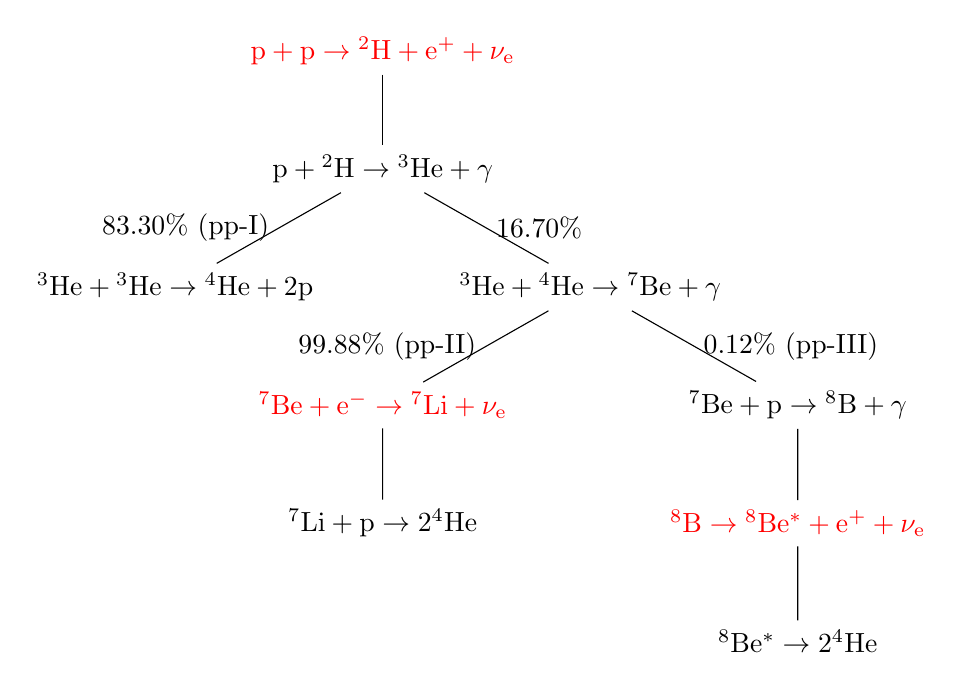
\begin{tikzpicture}[sibling distance=15em,
  every node/.style = {shape=rectangle,
    draw, align=center}
  edge from parent/.style = {draw, -latex},]]
  \node {\color{red}$\mathrm{p+p\to {}^2H + e^+ +\nu_e}$ }
    child { node {$\mathrm{p+{}^2H \to {}^3He + \gamma}$}
      child { node {$\mathrm{{}^3He+{}^3He \to {}^4 He + 2p }$}
          edge from parent node [left] {83.30\% (pp-I) } }
      child { node {$\mathrm{{}^3He+{}^4He \to {}^7 Be + \gamma }$}
        child { node {
\color{red}$\mathrm{{}^7Be + e^- \to {}^7Li + \nu_e}$
        }
        child { node { $\mathrm{{}^7Li + p \to 2{}^4He }$} }
        edge from parent node [left] {99.88\% (pp-II) } }
        child { node { $\mathrm{{}^7 Be + p \to {}^8 B + \gamma}$}
        child { node { \color{red}$\mathrm{{}^8B \to {}^8Be^* +e^+ +\nu_e}$ }
		child { node { $\mathrm{{}^8Be^* \to 2 {}^4He }$ } }}
        edge from parent node [right] {0.12\% (pp-III) } }
        edge from parent node [right] {16.70\%  } }};
\end{tikzpicture}
\end{adjustbox}
\caption{The pp chain reactions with the corresponding branching ratios. The branching ratios are taken from Ref.~\cite{Altmann2001}. }
\label{fig:pp_Chain_Branching}
\end{figure*}


% \begin{figure}[!hbtp]
% \centering
% 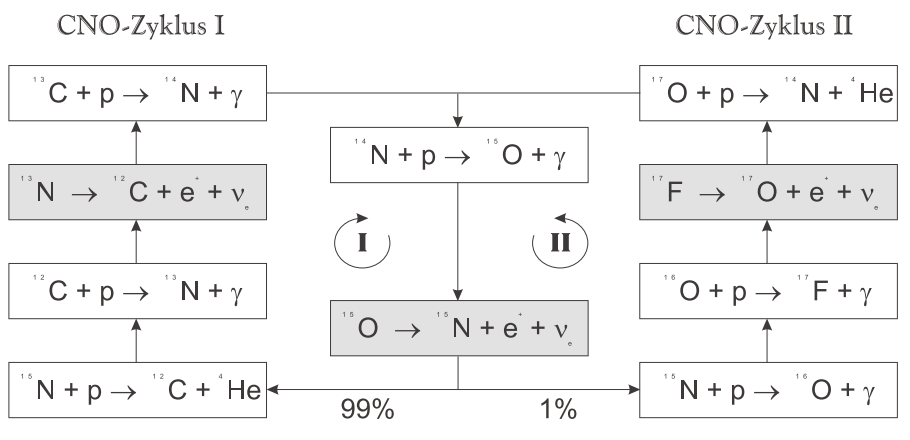
\includegraphics[width=\columnwidth]{chapters/assets/solar/cno_cycle.png}
% \caption{CNO cycle illustration~\cite{Adelberger2011a}.}
% \label{fig:cno_cycle}
% \end{figure}


Even without the knowledge of the detailed reactions, the conservation of the electric charge and the electron lepton number will lead to the overall neutrino production formula
\begin{equation}
\mathrm{4p+2e^- \to {}^4He + 2\nu_e }.
\end{equation}
It is important to notice that two neutrinos are emitted for each $\alpha$ particle, i.e., ${}^4\mathrm{He}$, produced in the Sun. Using this simple relation, we can estimate the neutrino number flux emitted by the Sun. The energy released during the production of each $\alpha$ particle is the difference between the initial and final rest masses of the particles,
\begin{equation}
Q=4m_p+2m_e-m_{\alpha}=26.7\mathrm{MeV},
\end{equation}
where the mass of the neutrinos are neglected. On average, each neutrino carries away an energy of $0.2\mathrm{MeV}$ and the rest of the energy is in the form of thermal energy $Q_\gamma=26.3\mathrm{MeV}$~\cite{Adelberger2011a}. %Energy flux density of solar photons near Earth is given by the solar constant $S_0$.
Since two neutrinos are emitted for the production of thermal energy $Q_\gamma$, the number flux of the solar neutrinos near the Earth is approximately
\begin{equation}
\Phi_\nu = \frac{2 S_0}{Q_\gamma} \approx 6\times 10^{10} \mathrm{cm^{-2}s^{-1}},
\end{equation}
where the solar constant $S_0$ is the energy flux of solar photons on the top of the Eath atmosphere.
%Neutrinos are hard to detect but a large number flux makes it possible to detect solar neutrinos~\cite{Cleveland1998,Lande2003,McDonald2013}.

% On the other hand, the solar neutrinos have a certain energy spectrum due to the composition of nuclear reactions. Inside our Sun, two additional reactions other than pp neutrinos also produce neutrinos which are called pep and hep neutrinos.
% \begin{itemize}
% \item pep neutrinos are produced in
% \begin{equation}
% \mathrm{p + e^- + p \to {}^2H +\nu_e},
% \end{equation}
% which only has a branching ratio 0.4\% instead of the 99.6\% of pp reaction.
% \item hep neutrinos are produced in
% \begin{equation}
% \mathrm{ {}^3He + p \to {}^4He + e^+ \nu_e },
% \end{equation}
% which has a branching ratio of $2\times 10^{-5}\%$. As a comparison, the $\mathrm{{}^3He + {}^3He}$ has a branching ratio $85\%$ and $\mathrm{{}^3He + {}^4He}$ has a branching ratio $15\%$.
% \end{itemize}


As the detection of neutrinos became feasible, Ray Davis and John Bahcall et al worked out the solar neutrino flux and led the Homestake experiment to measure the solar neutrinos. The results revealed that the neutrino flux detected was less than what was predicted by the standard solar model~\cite{Bahcall1973}. This is the solar neutrino problem. It is now known that the solution to the problem is related to the neutrino. The electron neutrinos produced in the solar core transform to other flavors while they travel to the Earth. This phonomenon is referred known as the flavor transformation of the neutrino, or neutrino oscillations. The theory of neutrino oscillations was first proposed by Pontecorvo in 1968~\cite{Pontecorvo1968}. The field of neutrino oscillations has grown significantly into a broad field in physics since then.



\section{Supernova Neutrinos}


Another astronomical source of neutrinos is the core-collapse supernova explosion. Massive stars with masses larger than 6−8 solar masses are very bright. However, violent delights have violent ends. When the core of a massive star runs out of nuclear fuel, it collapses under its own gravity. During the collapse, the inner core is compressed to almost nuclear density, which has a stiff equation of state. The materials falling onto the highly compressed inner core are bounced outward which generates a shock wave and may lead to an explosion. However, supernova simulations to date show that the shock wave itself is not always energetic enough to produce the explosion~\cite{Janka2016b}. In most cases, it stalls and becomes a standing accretion shock wave. To revive the shock, more energy has to be deposited behind the shock. A possible solution is to introduce reheating of the shock by neutrinos~\cite{Janka2016b}. In fact 99\% percent the energy released in a core-collapse supernova is carried away by neutrinos.
%Those explosions are the most luminous sources of neutrinos in the universe~\cite{Raffelt1996wa}.
In order to implement the neutrino-driven mechanism in computer simulations of supernovae, the flux and flavor content of the neutrinos have to be known everywhere behind the shock. Thus neutrino oscillations in dense matter become a key to the supernova explosion problem.

The average energy of the neutrinos $\langle E \rangle$ emitted during a supernova explosion is of the order of 10MeV~\cite{Janka2017}, and the neutrino luminosity at the early epoch is approximately $10^{52}\mathrm{ergs\cdot s^{-1}}$~\cite{Pejcha2012a}.
% The supernova explosion releases neutrinos with energy flux on the order of $10^{51}\mathrm{ergs\cdot s^{-1}}$~\cite{Bethe1985}.
Therefore, the number density of the neutrinos at the radius $R$ is
\begin{equation*}
   n \sim  10^{18} \mathrm{cm^{-3}} \left(\frac{100\mathrm{km}}{R}\right)^2 \left(\frac{10\mathrm{MeV}}{\langle E \rangle}\right).
\end{equation*}
% which corresponds to the number flux
% \begin{equation*}
%   \Phi \sim 10^{27} \mathrm{cm^{-2} s^{-1}}\left(\frac{100\mathrm{km}}{R}\right)^2 \left(\frac{10\mathrm{MeV}}{\langle E \rangle}\right).
% \end{equation*}
% Compared to the neutrino flux at the surface of the Sun, which is of the order $10^{15}\mathrm{cm^{-2} s^{-1}}$, supernova neutrinos is much denser.
It turns out that the ambient dense neutrino medium has a significant impact on neutrino oscillations, which has been intensely investigated in the last decade~\cite{Duan2010}.

Observation-wise, the neutrino signals from a galactic supernova can reveal a great amount of information about the physical conditions inside the supernova. In fact, the detection of supernova neutrinos is on the task list of the Deep Underground Neutrino Experiment (DUNE)~\cite{Kemp2017}.




\section{Organization of the Disseration}


% As we have seen, it is crucial to understand neutrino flavors.
The rest of the disseration is organized as follows.
In Chapter~\ref{chap:basics}, I will review neutrino oscillations in vacuum and in environments with smooth matter density profiles.
% Meanwhile, neutrino oscillations are ingredients of many other astrophysical, cosmological, and astronomical problems, such as neutron star mergers, dark matter, nucleosynthesis, etc. In order to gain a better understanding of neutrinos in these exotic environments, neutrino oscillations in dense matter background and dense neutrino background have to be thoroughly investigated. The seminal work by Mikheev--Smirnov--Wolfenstein proved neutrino interactions with matter background have significant effect on neutrino oscillations. They showed that neutrinos propagating through decreasing matter density experience a potential that alters the flavor conversions (MSW effect), which may also lead to maximum conversions between flavors~\cite{Mikheev:1986gs,wolf78,wolfensteinprd1979}. It is also know that neutrino oscillations in more general matter density profiles exhibit interesting phenomena. Resonances are found as the characteristic length scale in matter density profile and characteristic length scale of the neutrinos satisfies certain relations.
In Chapter~\ref{chap:matter}, I will discuss my work on neutrino oscillations in oscillatory matter profiles, which can be decomposed into Fourier modes and interpreted as a superposition of Rabi oscillations.
%Apart from dense matter background, neutrinos also interact with neutrinos themselves and introducing nonlinear dynamics. The neutrino self-interactions are analyzed using linear stability analysis.
In Chapter~\ref{chap:collective}, I will first review how neutrino self-interactions can cause a dense neutrino medium to oscillate collectively. Then I will discuss my study on the dispersion relations of the collective modes of neutrino oscillations.
%, as well as the dispersion relations in linear stability analysis. I will also discuss the neutrino halo problem. The halo problem exists because neutrino propagating out of dense matter medium will be scattered and forming a neutrino halo. Some of the neutrinos will propagate backward and interact with forward propagating neutrinos and alter the neutrino flavors. Mathematically speaking, the neutrino halo problem is a nonlocal boundary value problem. I will explain the numerical relaxation scheme that we developed, which we have proven to be a promising method to solve neutrino halo problem.
I will also discuss a premilinary work on neutrino oscillations when both forward and backward neutrino fluxes are present.
In Chapter~\ref{chap:conclusion}, I will summarize my work and discuss possible future directions of the field.

%!TEX root = ../dissertation.tex


\chapter{Neutrinos and Associated Particles}


This is chapter one \cite{Babu1992}.

%!TEX root = ../phd-thesis-lei-ma.tex
%!TeX spellcheck = en-US


\chapter{\label{chap:basics}General Principles of Neutrino Oscillations}

Since the flavor eigenstates of the neutrino are not the same as its propagation eigenstates, it can change flavor while it propagates.
In this chapter, I will use the two-flavor scheme to explain neutrino oscillations in some simple scenarios.\footnote{In most physical problems, the two-flavor scheme is a good approximation to the phenomena of neutrino oscillations. The two mass splitings between the three mass eigenstates are so different that the corresponding oscillations occur on very different length scales. On a given length scale, the two-flavor scheme captures the prominent features of the neutrino oscillations of the corresponding mass spliting.}
I will first discuss neutrino oscillations in vacuum. After explaining the general principles of neutrino oscillations in matter, I will show how the solar neutrino problem can be explained by neutrino oscillations. Finally, I will demonstrate the flavor isospin picture which can be used to visualize neutrino oscillations.


\section{\label{chap:basics-sec:vacuum-oscillations}Vacuum Oscillations}

Before carrying out the calculations, I can estimate the frequency of the oscillations of the neutrino between its flavors. In the natural units, frequency has the same dimension as energy.
% (see Appendix~\ref{chap:app-sec:conventions-subsec:units}).
Consider an electron neutrino with momentum $p$ which is a superposition of the two mass eigenstates $\ket{\nu_i}$ ($i=1,2$) with masses $m_i$, respectively. Since the neutrino masses are small, I can Taylor expand the energy of each mass eigenstate in terms of the corresponding mass:
\begin{align}
E_i & = \sqrt{m_i^2 + p^2 } \nonumber\\
& = p \sqrt{\frac{m_i^2}{p^2} + 1} \nonumber\\
& \approx p + \frac{1}{2} \frac{m_i^2}{p}.
\label{chap:basics-section:neutrinos-eqn:energy-taylor}
\end{align}
The first term in the above equation produces a global phase to the flavor wave function of the neutrino which does not affect neutrino flavor oscillations. The characteristic energy scale in the problem is the difference between the energies of the two mass eigenstates,
\begin{equation}
    \omega_{\mathrm v} = E_2-E_1 =  \frac{m_2^2-m_1^2}{2E} = \frac{\delta m^2}{2E},
    \label{chap:basics-section:neutrinos-eqn:qualitative-method-frequency}
\end{equation}
which turns out to be the vacuum oscillation frequency. Here $E=p$ is approximately the energy of the neutrino.

To work out the exact solution, I will utilize the Schr\"{o}dinger equation. First of all, the flavor eigenstates are denoted as $\ket{\nu_\alpha}$ where ${}_\alpha$ can be ${}_{\mathrm{e}}$ or ${}_{\mathrm{x}}$ for the electron flavor and the other flavor. The wave function of neutrino state $\ket{\nu}$ in the flavor basis, defined as
\begin{equation}
    \Psi^{(\ff)} = \begin{pmatrix}
        \psi^{(\ff)}_{\mathrm e} \\
        \psi^{(\ff)}_{\mathrm x}
    \end{pmatrix} = \begin{pmatrix}
        \braket{\nu_{\mathrm e}}{\nu} \\
        \braket{\nu_{\mathrm x}}{\nu}
    \end{pmatrix},
\end{equation}
is related to the wave function in the vacuum mass basis $\Psi^{(\vv)}$ through a unitary mixing matrix $\mathsf U$,
\begin{equation}
\Psi^{(\mathrm f)} = \mathsf{U}\Psi^{(\vv)},
\label{chap:vacuum-eqn:wavefunction}
\end{equation}
where the upper indices ${}^{(\vv)}$ and ${}^{(\ff)}$ are used to denote the corresponding bases. The mixing matrix can be expressed using the vacuum mixing angle $\theta_{\vv}$:
\begin{equation}
\mathsf{U} = \begin{pmatrix} \cos\theta_\vv & \sin \theta_\vv \\ -\sin \theta_\vv & \cos \theta_\vv \end{pmatrix}.
\end{equation}
In the vacuum mass basis, the neutrino has a free propagation Hamiltonian
\begin{equation}
\mathsf H^{(\vv)} = \begin{pmatrix} E_1 & 0 \\
0 & E_2
\end{pmatrix}.
\end{equation}
To the first order, the Hamiltonian becomes
\begin{align}
\mathsf H^{(\vv)} &\approx \frac{1}{2E} \begin{pmatrix}
m_1^2 & 0 \\
0 & m_2^2
\end{pmatrix} + E \mathsf{I} \nonumber \\
& =  \frac{1}{4E} \begin{pmatrix}
 - \delta m^2 & 0 \\
0 & \delta m^2
\end{pmatrix}  + \left(\frac{m_2^2 + m_1^2}{4E}  + E \right) \mathsf{I}.
\end{align}
Because a multiple of the identity matrix $\mathsf{I}$ gives only a global phase to the neutrino flavor wave function, I will neglect it from now on, and the vacuum Hamiltonian simplifies to
\begin{equation}
\mathsf H^{(\vv)} \to  \frac{\delta m^2}{4E} \begin{pmatrix}
-1 & 0 \\
0 & 1
\end{pmatrix} = -\frac{\delta m^2}{4E} \sigma_3 = -\frac{\omega_{\vv}}{2}\sigma_3,
\end{equation}
where
\begin{align}
\sigma_1 &=  \begin{pmatrix}
0 & 1 \\
1 & 0
\end{pmatrix}, &\sigma_2 &=  \begin{pmatrix}
0 & -\ii \\
\ii & 0
\end{pmatrix},  &\sigma_3 &=  \begin{pmatrix}
1 & 0 \\
0 & -1
\end{pmatrix}
\end{align}
are the three Pauli matrices.
The Schr\"{o}dinger equation has the following simple solution in the mass basis:
\begin{equation}
\Psi^{(\vv)}(t) = \begin{pmatrix}
c_1(0) e^{i \omega_\vv t/2 } \\
c_2(0) e^{ -i\omega_\vv t/2 }
\end{pmatrix}.
\end{equation}
% where the initial condition is
% \begin{equation}
% \Psi_v^{(v)}(0) = \begin{pmatrix}
% c_1(0) \\
% c_2(0)
% \end{pmatrix}.
% \end{equation}
Using Eqn.~\eqref{chap:vacuum-eqn:wavefunction}, I obtain the wave function in the flavor basis,
\begin{align}
\Psi^{(\ff)}(t) &= \mathsf{U}\Psi^{(\vv)}(t) \\
& = \begin{pmatrix} \cos\theta_\vv & \sin \theta_\vv \\ -\sin \theta_\vv & \cos \theta_\vv \end{pmatrix} \begin{pmatrix} c_1(0) e^{i\omega_\vv t/2 } \\
c_2(0) e^{ -i\omega_\vv t/2 }    \end{pmatrix} .
\label{chap:vacuum-eqn:wavefuncion-time}
\end{align}
Alternatively, I can also determine the Hamiltonian in the flavor basis first, which is
%then solve the Sch\"{o}dinger equation. I will not show the steps here, however, the Hamiltonian in flavor basis is presented for future use,
\begin{equation}
\mathsf H^{(\ff)} = \mathsf U \mathsf H^{(\vv)} \mathsf U^\dagger = -\frac{\omega_\vv}{2}\cos 2\theta_\vv \sigma_3 + \frac{\omega_\vv}{2} \sin 2\theta_\vv \sigma_1.
    \label{chap:basics-sec:vacuum-osc-eqn:hamiltonian-vacuum}
\end{equation}
By solving the Schr\"{o}dinger equation in the flavor basis, I will obtain the same wave function as in Eqn.~\eqref{chap:vacuum-eqn:wavefuncion-time}.

%In many astrophysical neutrino sources such as the solar core, electron neutrinos are the most abundant. Thus the initial condition is usually assumed to be electron flavor in the calculation which leads to the survival probability of electron flavor
The probability for a neutrino emitted in the electron flavor at time $t=0$ to be detected as the electron flavor at a later time $t$ is
\begin{equation}
P(t) = 1-\sin^2(2\theta_\vv)\sin^2\left( \frac{\omega_\vv t}{2} \right).
\end{equation}
Since the neutrino travels with approximately the speed of light, the electron neutrino survival probability at a distance $r$ from the source is
\begin{equation}
P(r) =  1-\sin^2(2\theta_\vv)\sin^2\left( \frac{\omega_\vv}{2} r \right).
\label{chap:basics-eqn:vacuum-electron-probability}
\end{equation}
%An important parameter in vacuum oscillations is the oscillation length of the neutrino flavor conversion which is $1/\omega_\vv$.This confirms our qualitative method result in Eqn.~\eqref{chap:basics-section:neutrinos-eqn:qualitative-method-frequency}.
I plot the above result in Fig.~\ref{chap:basics-section:neutrinos-fig:vacuum-2-flavor-osc} which clearly shows the oscillatory behavior. The oscillation length is determined by the characteristic energy scale $\omega_\vv$, which confirms our estimation in Eqn.~\eqref{chap:basics-section:neutrinos-eqn:qualitative-method-frequency}. The oscillation amplitude is determined by $\sin^2(2\theta_\vv)$.

\begin{figure}[htp]
    \centering
    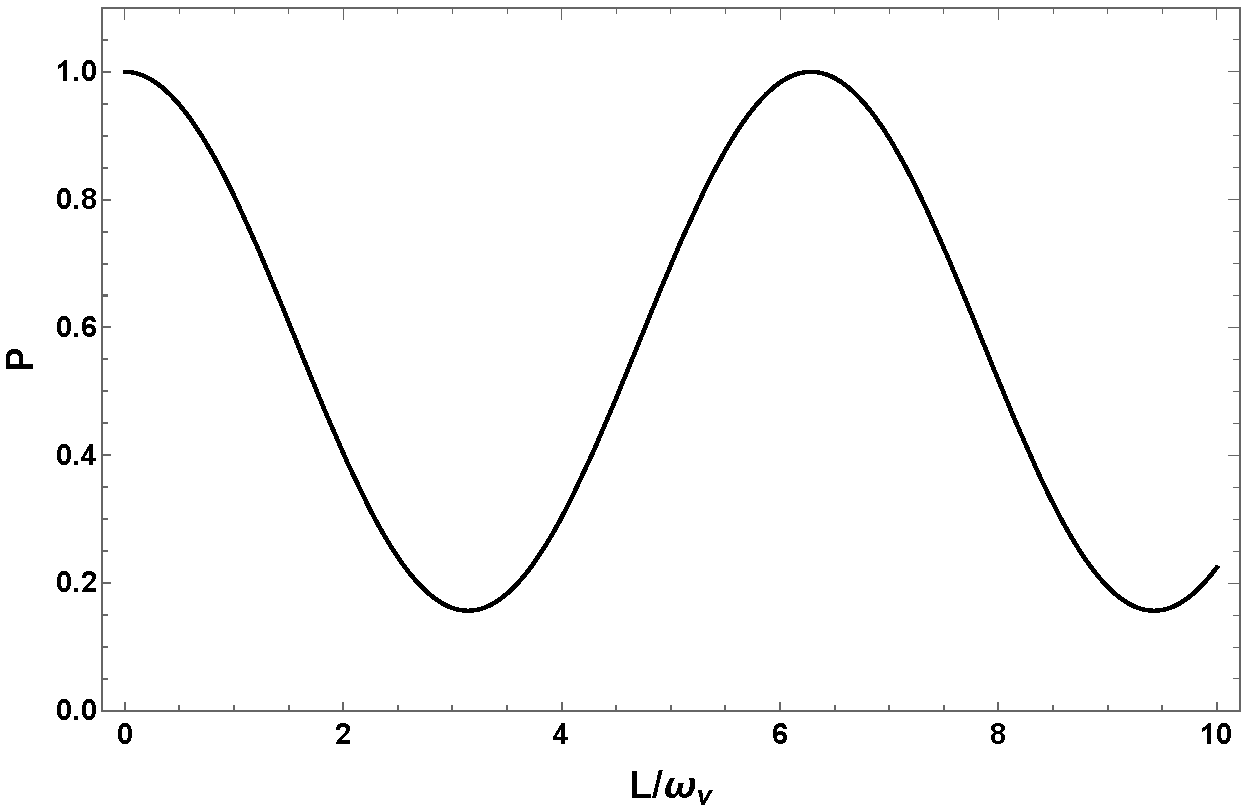
\includegraphics[width=0.8\textwidth]{chapters/assets/basics/neutrino-vaccum-osc-2-flavor.pdf}
    \caption{The electron flavor neutrino survival probability in vacuum oscillations as a function of distance $r$ which is measured in terms of vacuum oscillation frequency $\omega_\vv$. The mixing angle $\theta_\vv$ is given by $\sin^2\theta_\vv=0.30 \approx \sin^2 \theta_{12}$.}
    \label{chap:basics-section:neutrinos-fig:vacuum-2-flavor-osc}
\end{figure}



\begin{figure}[htp]
	\centering
	\begin{subfigure}[t]{0.48\textwidth}
		\centering
		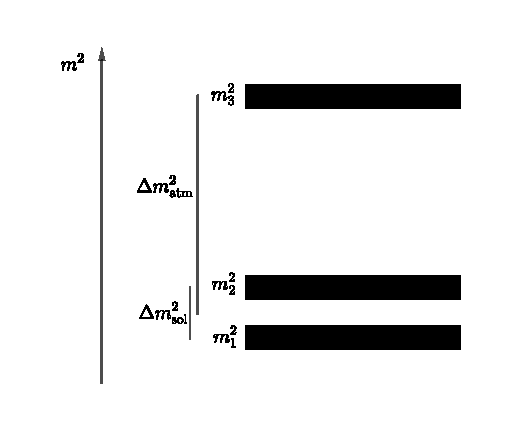
\includegraphics[width=\textwidth]{chapters/assets/basics/masses-nh}
		\caption{Normal hierarchy: the third mass is heavier than the first two.}
    \label{chap:basics-sec:flavor-isospin-pic-fig:masses-nh}
	\end{subfigure}
	\quad
	\begin{subfigure}[t]{0.48\textwidth}
		\centering
		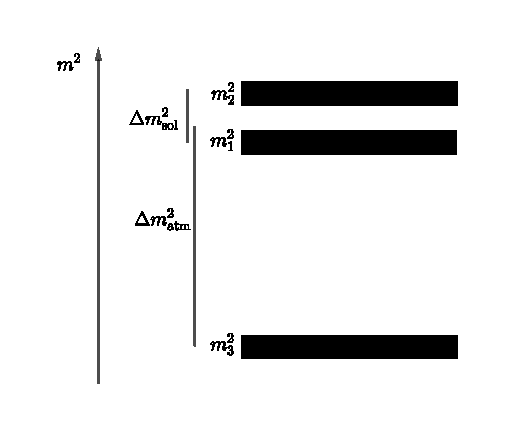
\includegraphics[width=\textwidth]{chapters/assets/basics/masses-ih}
		\caption{Inverted hierarchy: the third mass is smaller than the first two.}
    \label{chap:basics-sec:flavor-isospin-pic-fig:masses-ih}
	\end{subfigure}
	\caption{The order of the three neutrino masses. The difference between the first two masses is responsible for solar neutrino oscillations, and the difference between the third mass and the first two is responsible for atmospheric neutrino oscillations.}
    \label{chap:basics-sec:flavor-isospin-pic-fig:masses}
\end{figure}

\begin{figure}[htbp]
    \centering
    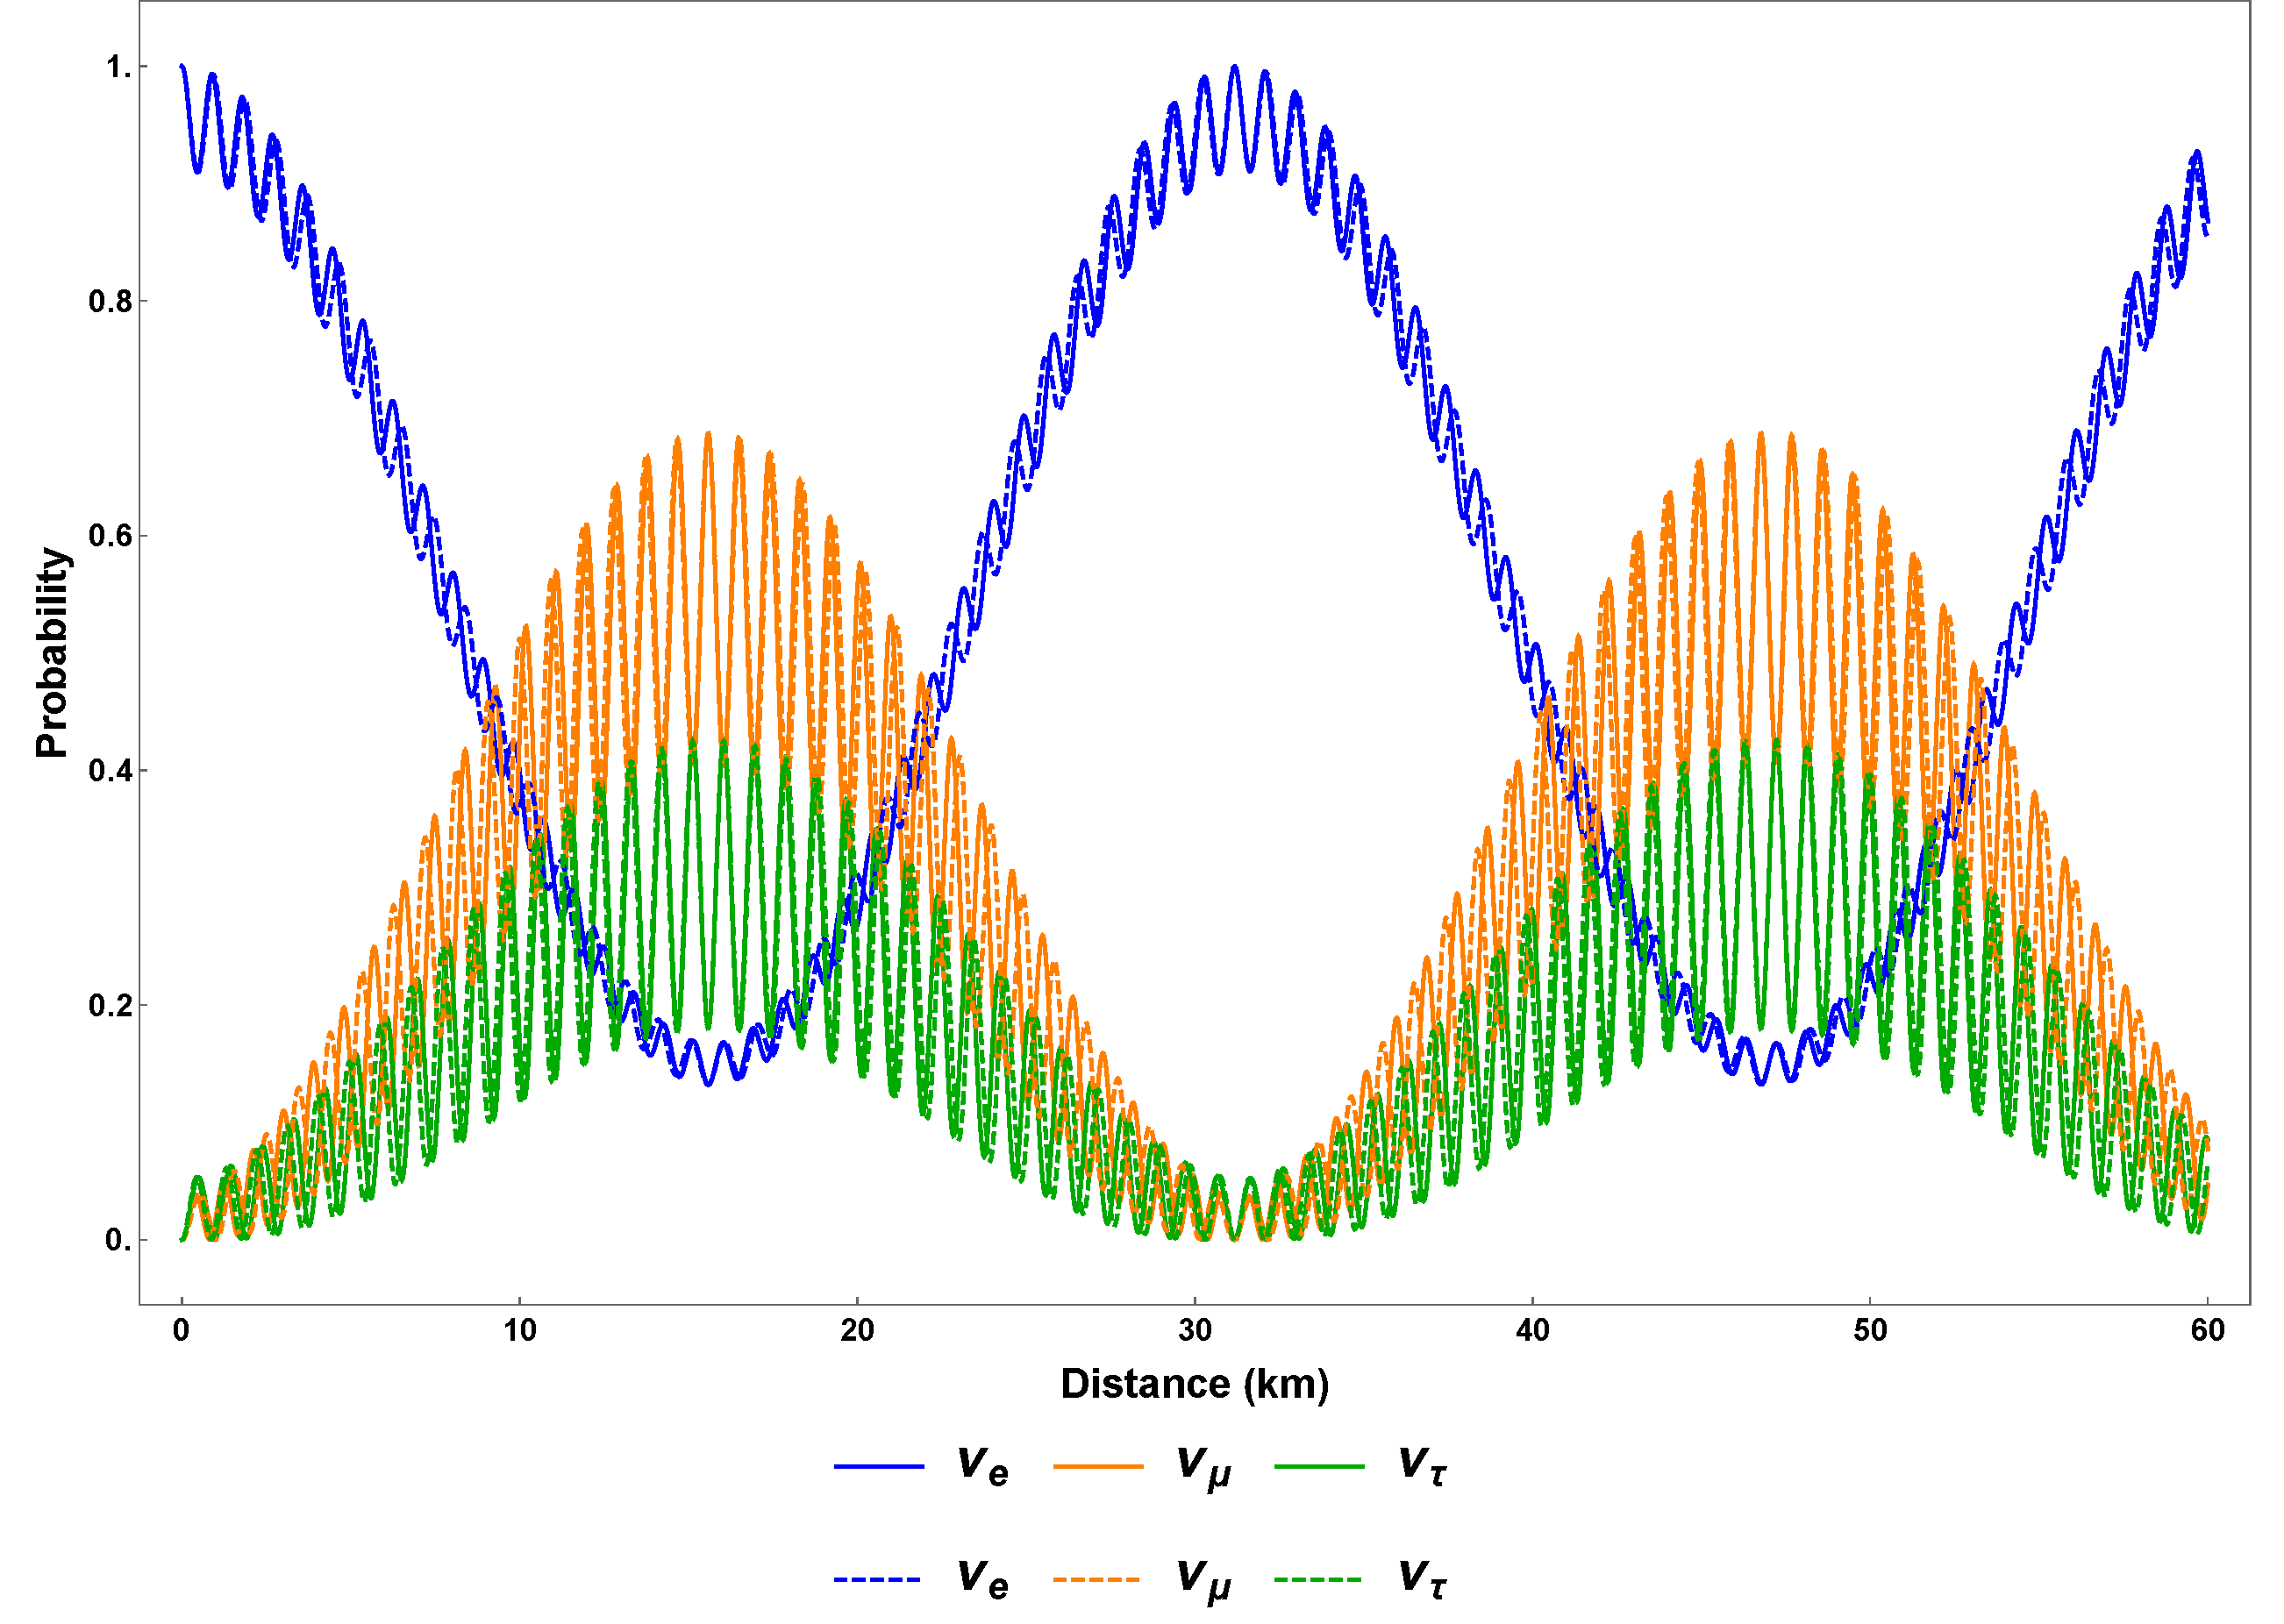
\includegraphics[width=\textwidth]{chapters/assets/basics/vacuum-oscillations-3-flavor.pdf}
    \caption{The probabilities for a $1\mathrm{MeV}$ neutrino, which is in the electron flavor initially, in different flavors as functions of the distance in vacuum. The solid lines represent the normal hierarchy and the dashed lines represent the inverted hierarchy. The mixing angles are $\sin^2\theta_{12}=0.30$, $\sin^2\theta_{13}=0.023$, and $\sin^2\theta_{23}=0.41$, respectively, and the mass differences are $\delta m_{21}^2 = 7.9\times 10^{-5}\mathrm{eV^2}$ and $\delta m^2_{23}=2.7\times 10^{-3}\mathrm{eV^2}$.}
    \label{chap:basics-section:neutrinos-fig:vacuum-3-flavor-osc}
\end{figure}


In nature, there are three neutrino flavors and, correspondingly, three neutrino mass eigenstates as shown in Fig.~\ref{chap:basics-sec:flavor-isospin-pic-fig:masses}. Because there are two different characteristic energy scales, $\omega_{\vv,21}=\delta m_{21}^2/2E$ and $\omega_{\vv,32}=\delta m_{31}^2/2E$, two oscillation periods should occur, as shown in Fig.~\ref{chap:basics-section:neutrinos-fig:vacuum-3-flavor-osc}. The fast oscillations are determined by the larger energy scale, $\omega_{\vv,32}$, while the slow oscillations are determined by the smaller one $\omega_{\vv,21}$. For the inverted neutrino mass hierarchy (with $m_3 < m_1 < m_2$), the oscillation frequencies are the same as in the normal mass hierarchy (with $m_3>m_2>m_1$) since they have the same characteristic energy scales. However, they will develop different phases during oscillations.

\clearpage

\section{\label{chap:basics-sec:oscillations-matter}Neutrino Oscillations in Matter}

\begin{figure}[htbp]
\centering
	\begin{subfigure}[t]{0.40\textwidth}
		\centering
		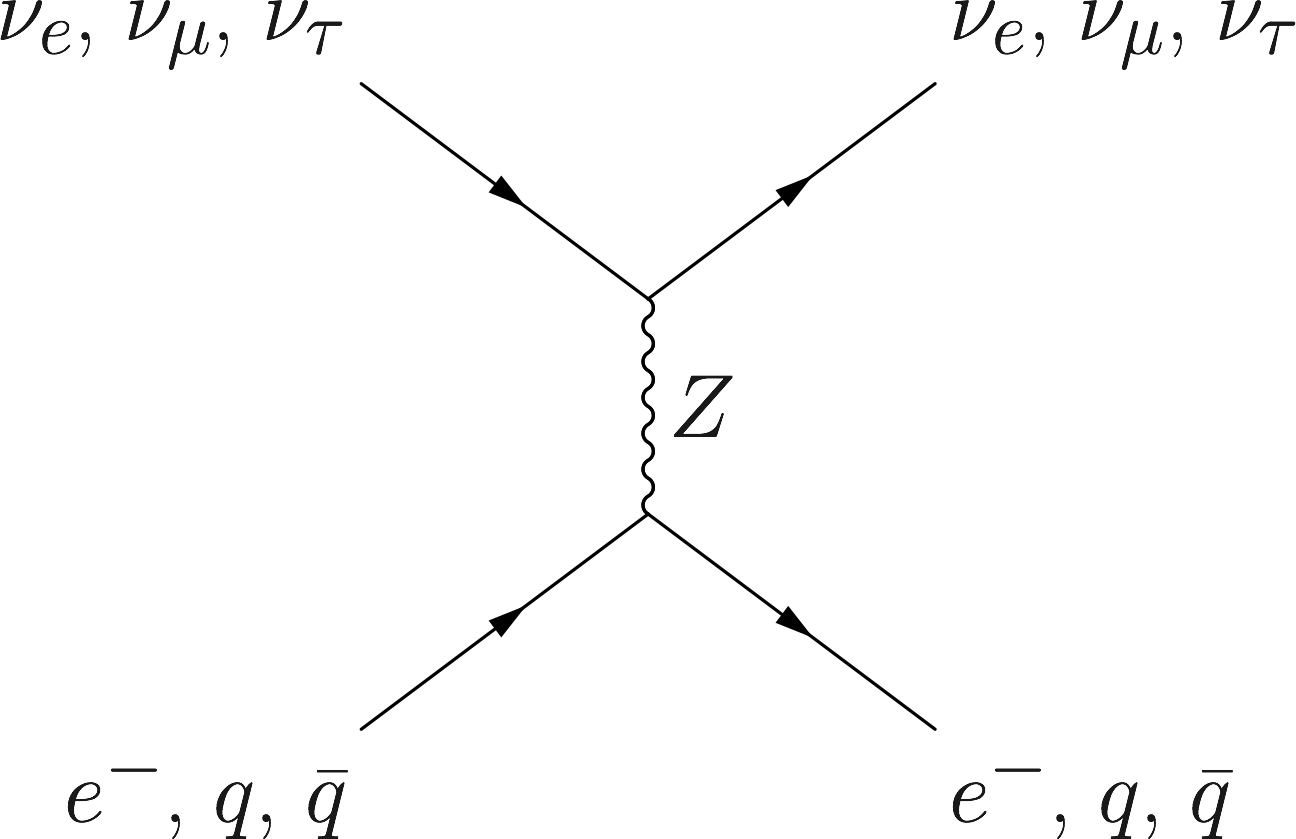
\includegraphics[height=0.2\textheight]{chapters/assets/matter/neutral-current.png}
    \caption{  }
		% \caption{Neutral current interaction between $\nu_{\mathrm e}$, $\nu_{\mu}$, $\nu_{\tau}$, and $e^{-}$. Neutral current interaction is mediated by Z bosons.}
    \label{chap:matter-fig:nc}
	\end{subfigure}%
  \qquad
	\begin{subfigure}[t]{0.40\textwidth}
		\centering
		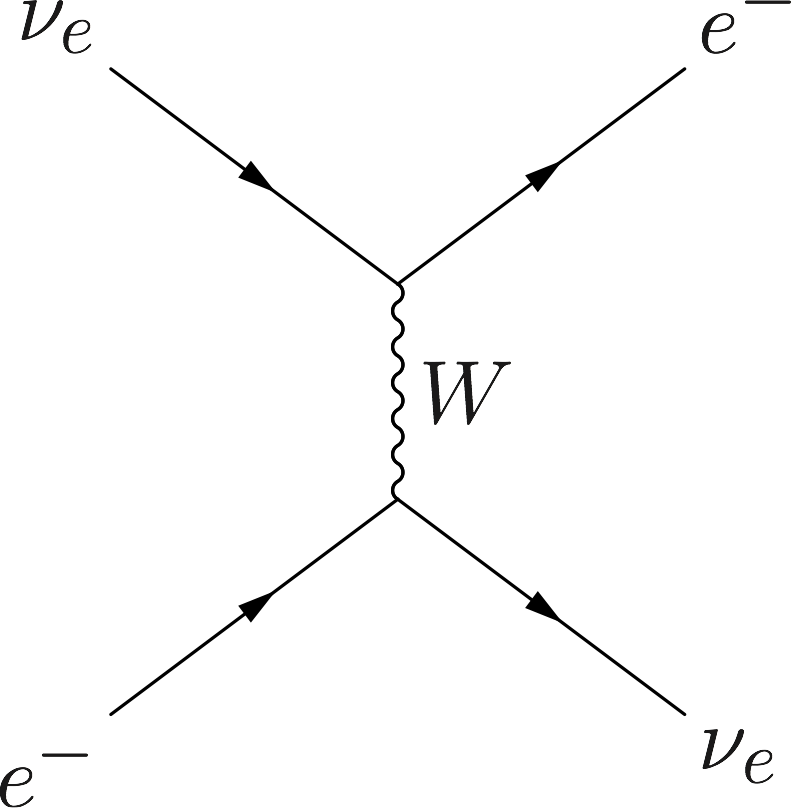
\includegraphics[height=0.2\textheight]{chapters/assets/matter/charged-current.png}
    \caption{  }
		% \caption{charged current interaction between $\nu_{\mathrm e}$ and $e^{-}$. Charged current interaction is mediated by W bosons.}
    \label{chap:matter-fig:cc}
	\end{subfigure}
	\caption{
  (a) The neutral current weak interaction does not distinguish between neutrino flavors and has no impact on neutrino oscillations. (b) The electron flavor neutrino acquires a unique refractive index contribution from the charged current weak interaction with ambient electrons.
  }
    \label{chap:matter-fig:nc-cc}
\end{figure}

In many astrophysical environments such as stars and core-collapse supernovae, neutrinos are mostly produced at the center of the environments and propagate through the dense matter envelope. Although this matter envelope is essentially transparent to neutrinos, the refractive indices of the neutrinos in matter are different than those in vacuum.\footnote{The word ``matter" in this dissertation refers to ordinary matter composed of electrons, positrons, nucleons and nuclei. I assume that the temperature and density of the environment are not high enough to produce muons and tau particles. I will discuss the effect of the dense neutrino medium in Chapter~\ref{chap:collective}.} Because the neutral current weak interaction does not distinguish between neutrino flavors (see Fig.~\ref{chap:matter-fig:nc}), it has no impact on neutrino oscillations, and I will ignore it from now on. Meanwhile, the electrons and positrons in matter will cause electron flavor neutrinos to have refractive indices different than the neutrinos of other flavors through the charged current weak interaction (see Fig.~\ref{chap:matter-fig:cc}).
% One of the significant matter effect on neutrino flavor oscillations is the Mikheyev-Smirnov-Wolfenstein (MSW) effect~\cite{Mikheev:1986gs,wolf78,wolfensteinprd1979}, which is used to explain the deficit of electron flavor neutrino flux, as know as the solar neutrino problem~\cite{kuo1989,Petcov2002}. Later developments on the theories of matter effect revealed the parametric resonance of neutrino flavor oscillations due to fluctuations in matter density~\cite{Krastev1989,Akhmedov2000}, which is the neutrino analog of transitions between energy levels as a result of external optical stimulation. Parametric resonance is different from the MSW effect since it involves the parameters of the matter density, which is usually the period of matter density fluctuations. It has also be shown that neutrinos passing through the Earth can experience parametric resonance~\cite{Akhmedov1999, Petcov1998b}.
%Flavor conversion occurs as long as their propagation eigenstates are different from their flavor eigenstates. Since the neutral current interactions between the neutrinos and the matter is independent of the flavors, as shown in Fig.~\ref{chap:matter-fig:nc}, I only include the charged current interactions in the Hamiltonian, which is an effective potential for electron flavor.
This leads to an effective potential
\begin{equation}
\mathsf V^{(\ff)} = \frac{\sqrt{2}G_{\mathrm F} n_{\mathrm e} }{2}  \sigma_3,
\label{chap:basics-sec:oscillations-matter-eqn:effective-pot}
\end{equation}
where $G_{\mathrm F}=1.17\times 10^{-5}\mathrm{GeV^{-2}}$ is Fermi constant and $n_{\mathrm e}$ is net number density of the electron. As usual, I have ignored the trace terms in the above expression.

The Hamiltonian with the matter effect is the combination of Eqn.~\eqref{chap:basics-sec:vacuum-osc-eqn:hamiltonian-vacuum} and Eqn.~\eqref{chap:basics-sec:oscillations-matter-eqn:effective-pot}:
% \begin{equation}
% \mathsf H^{(\ff)} = \frac{ \omega_\vv }{2}\begin{pmatrix} -\cos 2\theta_\vv & \sin 2 \theta_\vv \\ \sin 2\theta_\vv & \cos 2\theta_\vv  \end{pmatrix},
% \end{equation}
% where we used the result of flavor basis vacuum oscillation Hamiltonian
% \begin{align}
% \mathsf H_\vv^{(\ff)}& = \mathsf{U} \mathsf H_\vv \mathsf{U}^\dagger \\
% &= \frac{ \omega_\vv }{2}\begin{pmatrix} -\cos 2\theta_\vv & \sin 2 \theta_\vv \\ \sin 2\theta_\vv & \cos 2\theta_\vv  \end{pmatrix}.
% \end{align}
\begin{equation}
\mathsf H^{(\ff)} = \left(\frac{\lambda}{2} -\frac{ \omega_\vv }{2} \cos 2\theta_\vv \right) {\sigma}_3  + \frac{ \omega_\vv }{2} \sin 2\theta_\vv {\sigma}_1,
\label{chap:basics-sec:msw-eqn:hamiltonian-matter-effect}
\end{equation}
where
\begin{equation}
  \lambda = \sqrt{2}G_{\mathrm F} n_{\mathrm e}.
  \label{chap:basics-sec:oscillations-matter-eqn:lambda}
\end{equation}
Due to the off-diagonal terms in $\mathsf H^{(\ff)}$, the neutrino will experience oscillations in flavor. A resonance with the maximum flavor mixing occurs when the diagonal terms of $\mathsf H^{(\ff)}$ vanish, i.e.,
\begin{equation}
\frac{\lambda}{2} -\frac{ \omega }{2} \cos 2\theta_\vv  = 0,
\label{chap:basics-eqn:msw-resonance}
\end{equation}
which gives the Mikheyev--Smirnov--Wolfenstein (MSW) resonance condition.


\section{\label{chap:matter-sec:solar-neutrinos}Neutrino Oscillations in the Sun}


% \section{\label{chap:basics-sec:msw}Mikheyev--Smirnov--Wolfenstein Effect}

The neutrinos produced in the solar core experience decreasing matter density as they travel outward through the Sun. The neutrino propagation eigenstates are different from the flavor states in general~\cite{wolf78}.
%The importance of matter effect to our understanding of solar neutrinos is that it modifies the oscillations, depending on the matter density variation.
Because the density change inside the Sun is not dramatic, the flavor quantum states of the neutrinos will evolve adiabatically inside the Sun.

\begin{figure}[htbp]
\centering
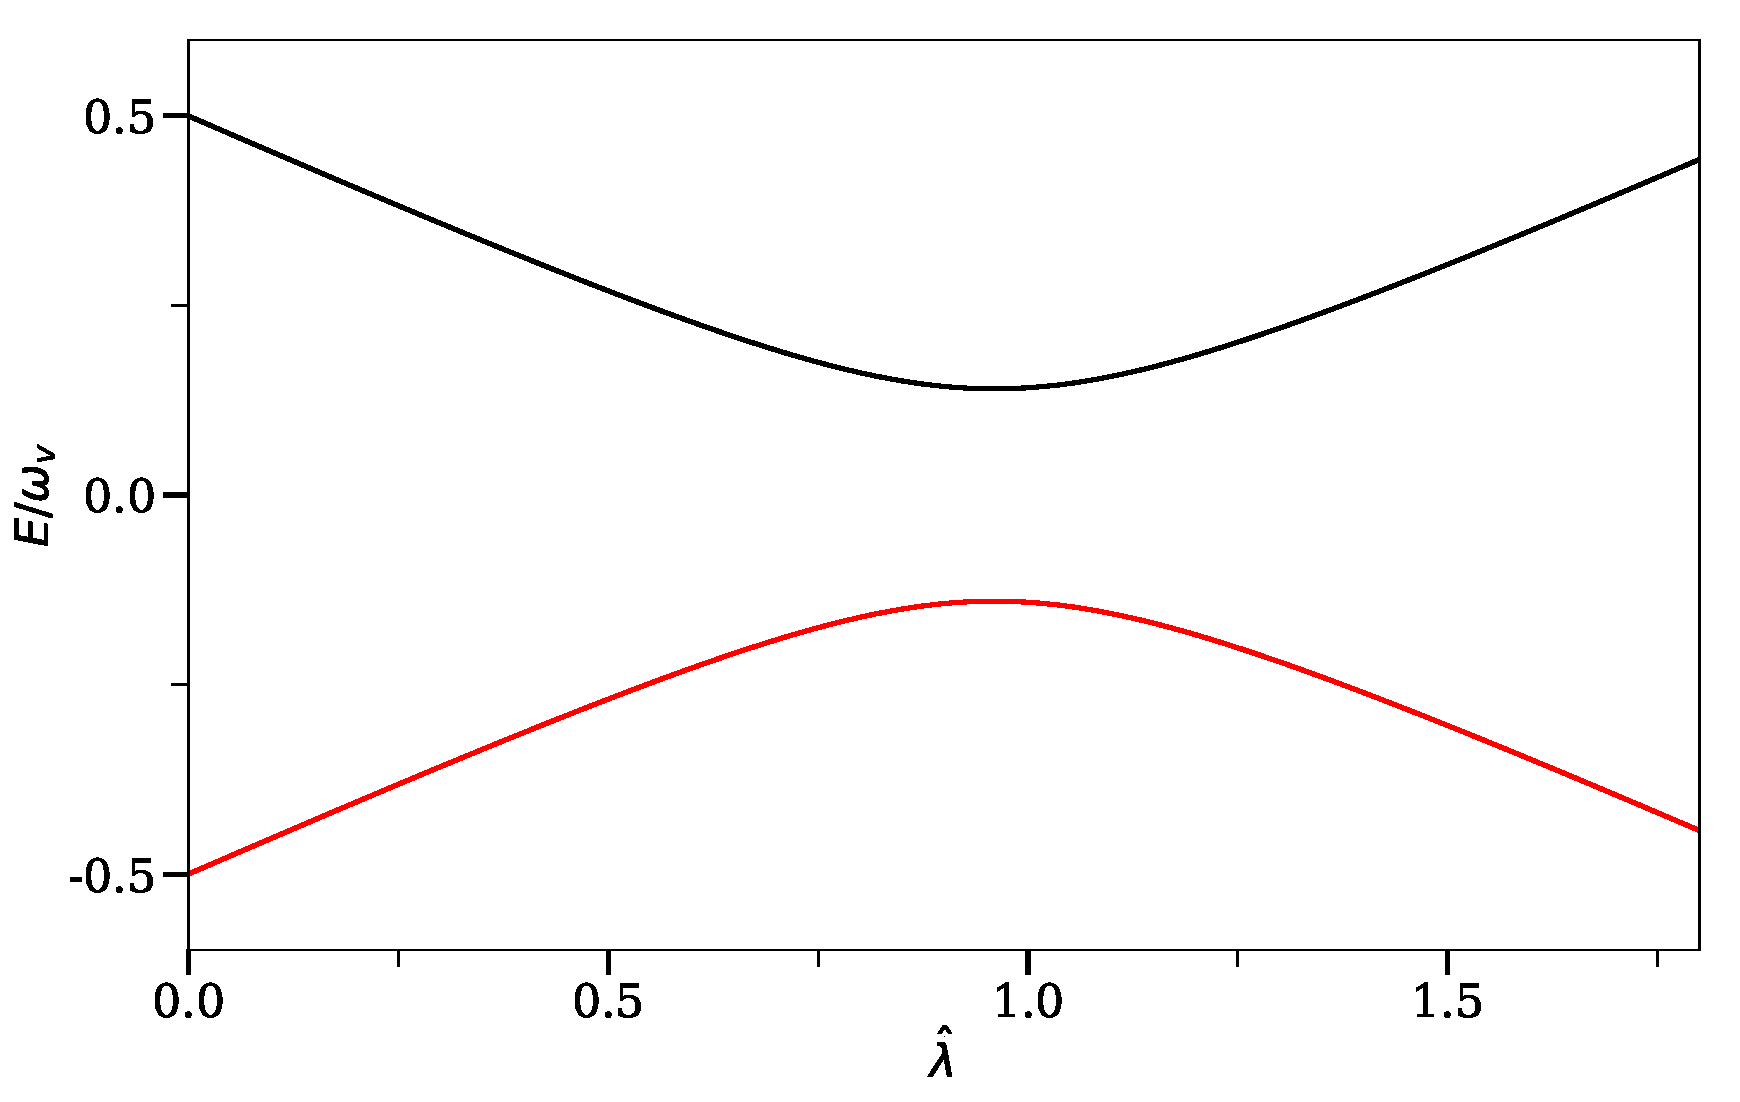
\includegraphics[width=0.7\columnwidth]{chapters/assets/matter/mswEnergyLevels}
\caption{The two eigenvalues of the neutrino Hamiltonian as functions of matter potential $\hat\lambda$. I have used $\sin^2\theta_\vv = 0.02 \approx \sin^2 \theta_{13}$.}
\label{fig:mswEnergyLevels}
\end{figure}

The values of the instantaneous eigenstates of the Hamiltonian, known as the ``Heavy'' and ``Light'' states, are
\begin{align}
\varepsilon_{\mathrm H} &= \frac{\omega_\vv}{2}\sqrt{ \hat\lambda +1 -  2\hat\lambda \cos 2\theta_\vv }, \\
\varepsilon_{\mathrm L} &= -\frac{\omega_\vv}{2}\sqrt{ \hat\lambda +1 -  2\hat\lambda \cos 2\theta_\vv },
\end{align}
% which means that the instantaneous eigenstates and eigenvectors of Hamiltonian is good enough for the time dependent Schr\"{o}dinger equation.
where
\begin{align}
\hat\lambda & = \frac{\lambda}{\omega_\vv}.
\end{align}
In Fig.~\ref{fig:mswEnergyLevels}, I show the two eigenvalues of the neutrino Hamiltonian as functions of the matter potential $\hat \lambda$.

For a very high matter density, the heavy state of the neutrino $\ket{\nu_{\mathrm H}}$ is almost the same as $\ket{\nu_{\ee}}$. As the matter density decreases, $\ket{\nu_{\mathrm H}}$ becomes a mixture of different neutrino flavors. As the neutrino reaches the surface of the Sun, where the matter density is approximately zero, $\ket{\nu_{\mathrm H}}$ is about the same as vacuum mass eigenstate $\ket{\nu_{2}}$. As a result, the electron flavor neutrinos produced at the solar core are partially converted to other flavors as they reach the surface of the Sun. This explains the solar neutrino problem.
% The MSW resonance occurs at $n_{\mathrm e} = 2\omega_\vv \cos(2\theta_\vv)/\sqrt{2}G_{\mathrm F}$.
%Neutrinos with different energies will encounter the MSW resonance at different matter densities, which will significantly reshape the neutrino energy spectra.
% Even though only the electron flavor neutrinos are produced in the Sun, the neutrino flavor conversion to the other flavors is enhanced by the matter interactions, in addition to the vacuum oscillation.
%The exact neutrino flavor conversion is much more complicated than the MSW effect.
% As an approximation, the MSW transition is good enough for the solar neutrinos flavor oscillations~\cite{Lopes2013a}.

% One of the interesting fact about MSW effect is the MSW triangle shown in Fig.~\ref{chap:basics-sec:msw-fig:msw-triangle}. The survival probability of the electron flavor neutrinos is plotted against $\log (\lambda/\omega_\vv)$ and $\log (\sin^2 2\theta_\vv)$. Qualitatively speaking, large conversion happens when matter density is not too small since a sufficient central potential is required for the level crossing. This leads to the triangle shape of the low survival probability region.
%
% \begin{figure}[htbp]
%     \centering
%     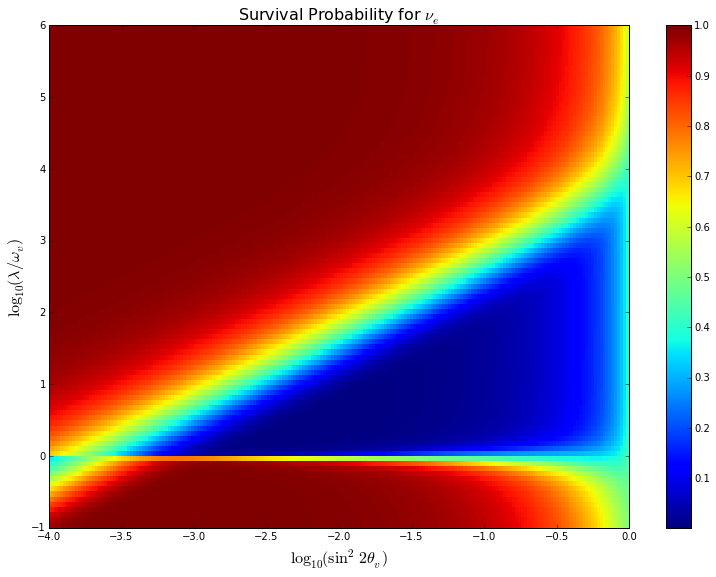
\includegraphics[width=0.9\textwidth]{chapters/assets/basics/msw-triangle.png}
%     \caption{MSW triangle. The horizontal axis is related to the the mixing angles, and the vertical axis is related to the matter potential in the center of the Sun. The colors are the survival probabilities of electron flavor. The region of large conversions, or small survival probabilities, forms a triangle. The larger the mixing angle, the larger range of matter potential for large conversions.}
%     \label{chap:basics-sec:msw-fig:msw-triangle}
% \end{figure}





% \section{\label{chap:matter-sec:flavor-isospin}Flavor Isospin Formalism}













\section{\label{chap:basics-sec:flavor-isospin-pic}Flavor Isospin Formalism}


\begin{figure}
    \centering
    \vspace*{-10pt}
    \includegraphics[width=\textwidth]{chapters/assets/basics/flavor-isospin-illus}
    \caption{In the flavor isospin picture, a flavor isospin pointing upward, i.e., along the third axis in flavor space, indicates that the neutrino is in the electron flavor, while the downward direction indicates the other flavor, such as the muon flavor.}
    \label{chap:basics-sec:flavor-isospin-pic-fig:flavor-isospin-illus}
\end{figure}

The Hamiltonian for two-flavor neutrino oscillations describes a two-level quantum system. It is known that two-level quantum systems can be visualized using the Bloch sphere. In the realm of neutrino physics, the neutrino flavor isospin was introduced for such purpose~\cite{Duan2006b}.


Every two-by-two Hermitian matrix can be expanded in the quaternion basis. For example, the Hamiltonian for neutrino oscillations in vacuum (in the flavor basis) can be written as
\begin{equation}
\mathsf H^{(\ff)} = - \frac{\vec{\sigma} }{2}\cdot {\vec{H}},
\end{equation}
where
\begin{align}
{\vec H} =  \omega_\vv\begin{pmatrix}
 \sin \theta_\vv\\
0\\
\cos 2\theta_{\mathrm v}
\end{pmatrix},
\end{align}
which is a vector of length $\omega_{\mathrm v}$ and tilted away from the third axis by angle $2\theta_{\mathrm v}$.
Throughout the dissertation, I will use ``$\vec{\phantom{x~}}$" to denote a vector in flavor space.
The flavor quantum state of the neutrino is represented by its flavor isospin which is defined as
\begin{equation}
    \vec s = {\Psi^{(\ff)}}^{\dagger} \frac{\vec{\sigma} }{2} \Psi^{(\ff)}.
\end{equation}
As shown in Fig.~\ref{chap:basics-sec:flavor-isospin-pic-fig:flavor-isospin-illus}, the direction of the flavor isospin in flavor space shows the flavor content of the neutrino. A flavor isospin pointing ``upward'' in flavor space, i.e., along the direction of the third axis, denotes the electron flavor by definition.
Correspondingly, the equation of motion for the flavor isospin describes its precession around the vector $\vec{H}$,
\begin{equation}
\dot{\vec{s}} = {\vec{s}} \times \vec{H},
\label{chap:basics-sec:flavor-isospin-pic-eqn:eom-precession}
\end{equation}
where $\dot{\phantom{s}}$ indicates the time derivative.
In the flavor isospin formalism, the electron flavor survival probability is
\begin{equation}
P = \frac{1}{2} + s_3,
\label{chap:basics-sec:flavor-isospin-pic-eqn:probability-flavor}
\end{equation}
where $s_3$ is the third component of the flavor isospin.
\begin{figure}[htbp]
    \centering
    % \vspace*{-20pt}
    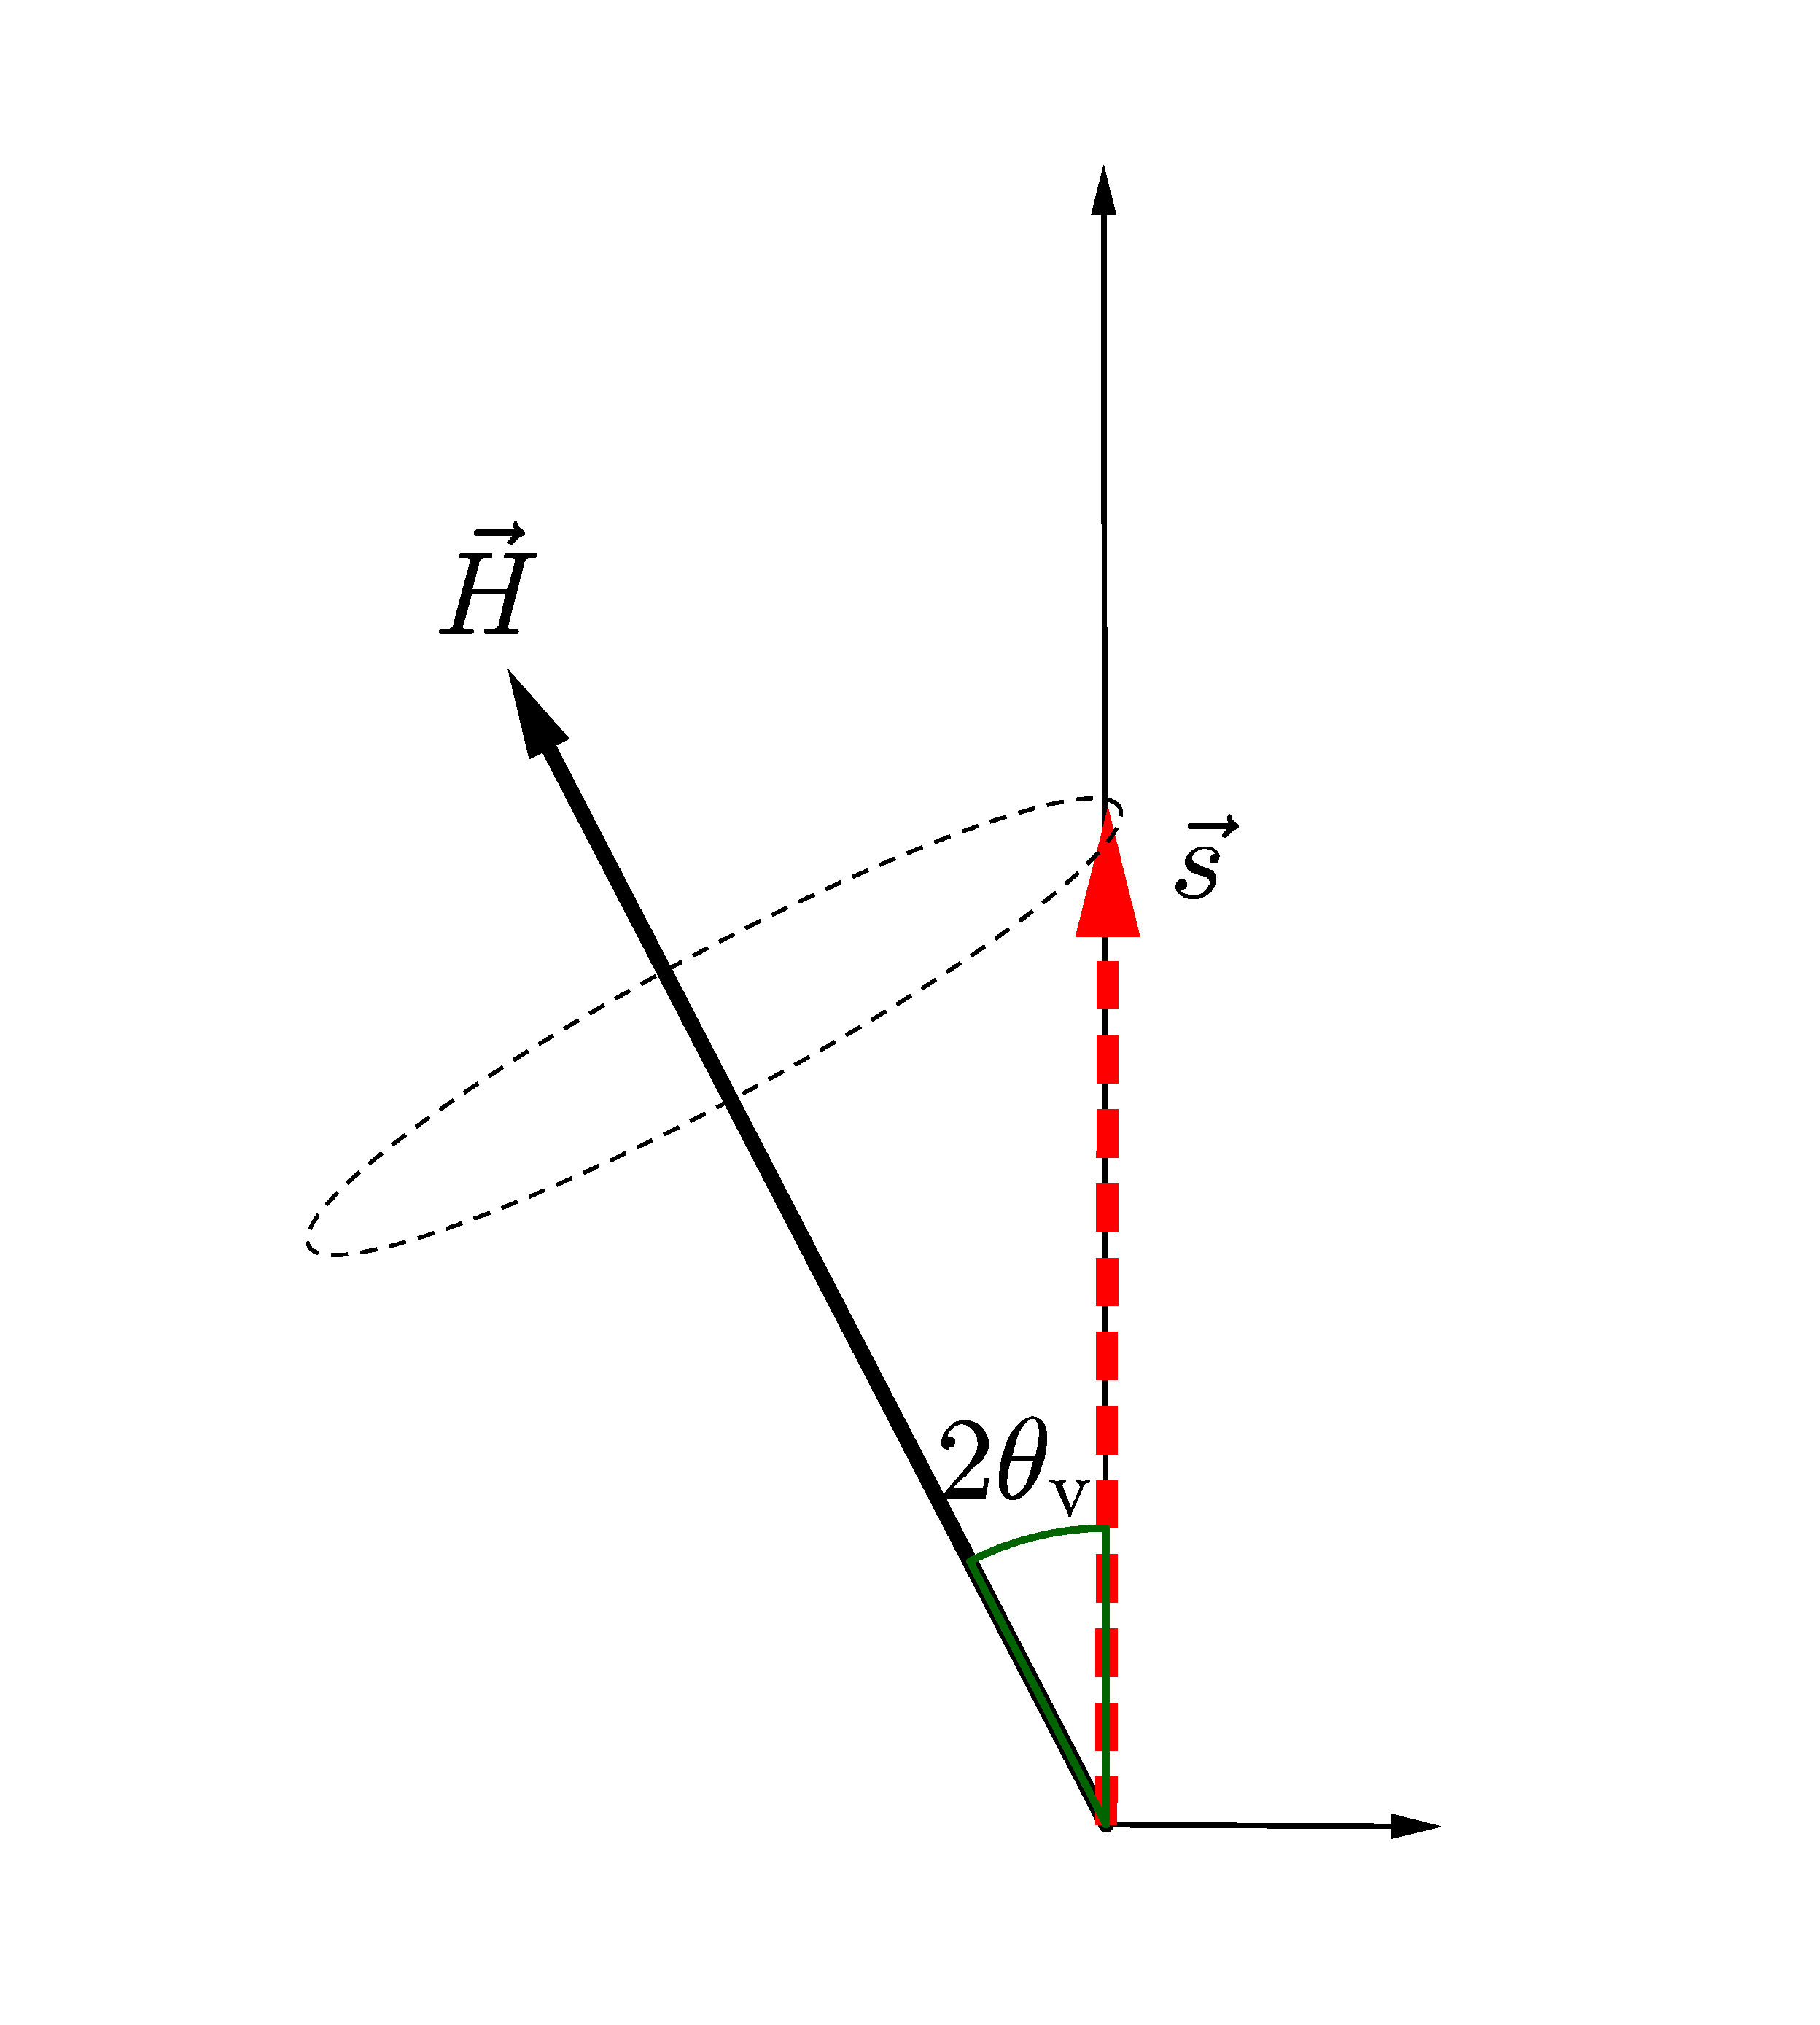
\includegraphics[width=0.6\textwidth]{chapters/assets/basics/flavor-isospin-vac-osc}
    \caption{Vacuum oscillations in the flavor isospin picture. The flavor isospin of a neutrino starting with the electron flavor precesses around the static ``Hamiltonian vecto
    r" $\vec H$, which gives a periodic flavor oscillation according to Eqn.~\eqref{chap:basics-eqn:vacuum-electron-probability}.}
    \label{chap:basics-sec:flavor-isospin-pic-fig:flavor-isospin-vac-osc}
\end{figure}
Therefore, the precession of the flavor isospin corresponds to a periodic oscillation between the two neutrino flavors (see Fig.~\ref{chap:basics-sec:flavor-isospin-pic-fig:flavor-isospin-vac-osc}).
%Eqn.~\eqref{chap:basics-sec:flavor-isospin-pic-eqn:eom-precession} depicts the precession of the flavor isospin for a neutrino which starts with the electron flavor and propagates in vacuum.
The oscillation frequency can be trivially read out from Eqn.~\eqref{chap:basics-sec:flavor-isospin-pic-eqn:eom-precession}:
\begin{equation}
\omega_\vv = \lvert \vec{H} \rvert.
\end{equation}




\begin{figure}[htbp]
    \centering
    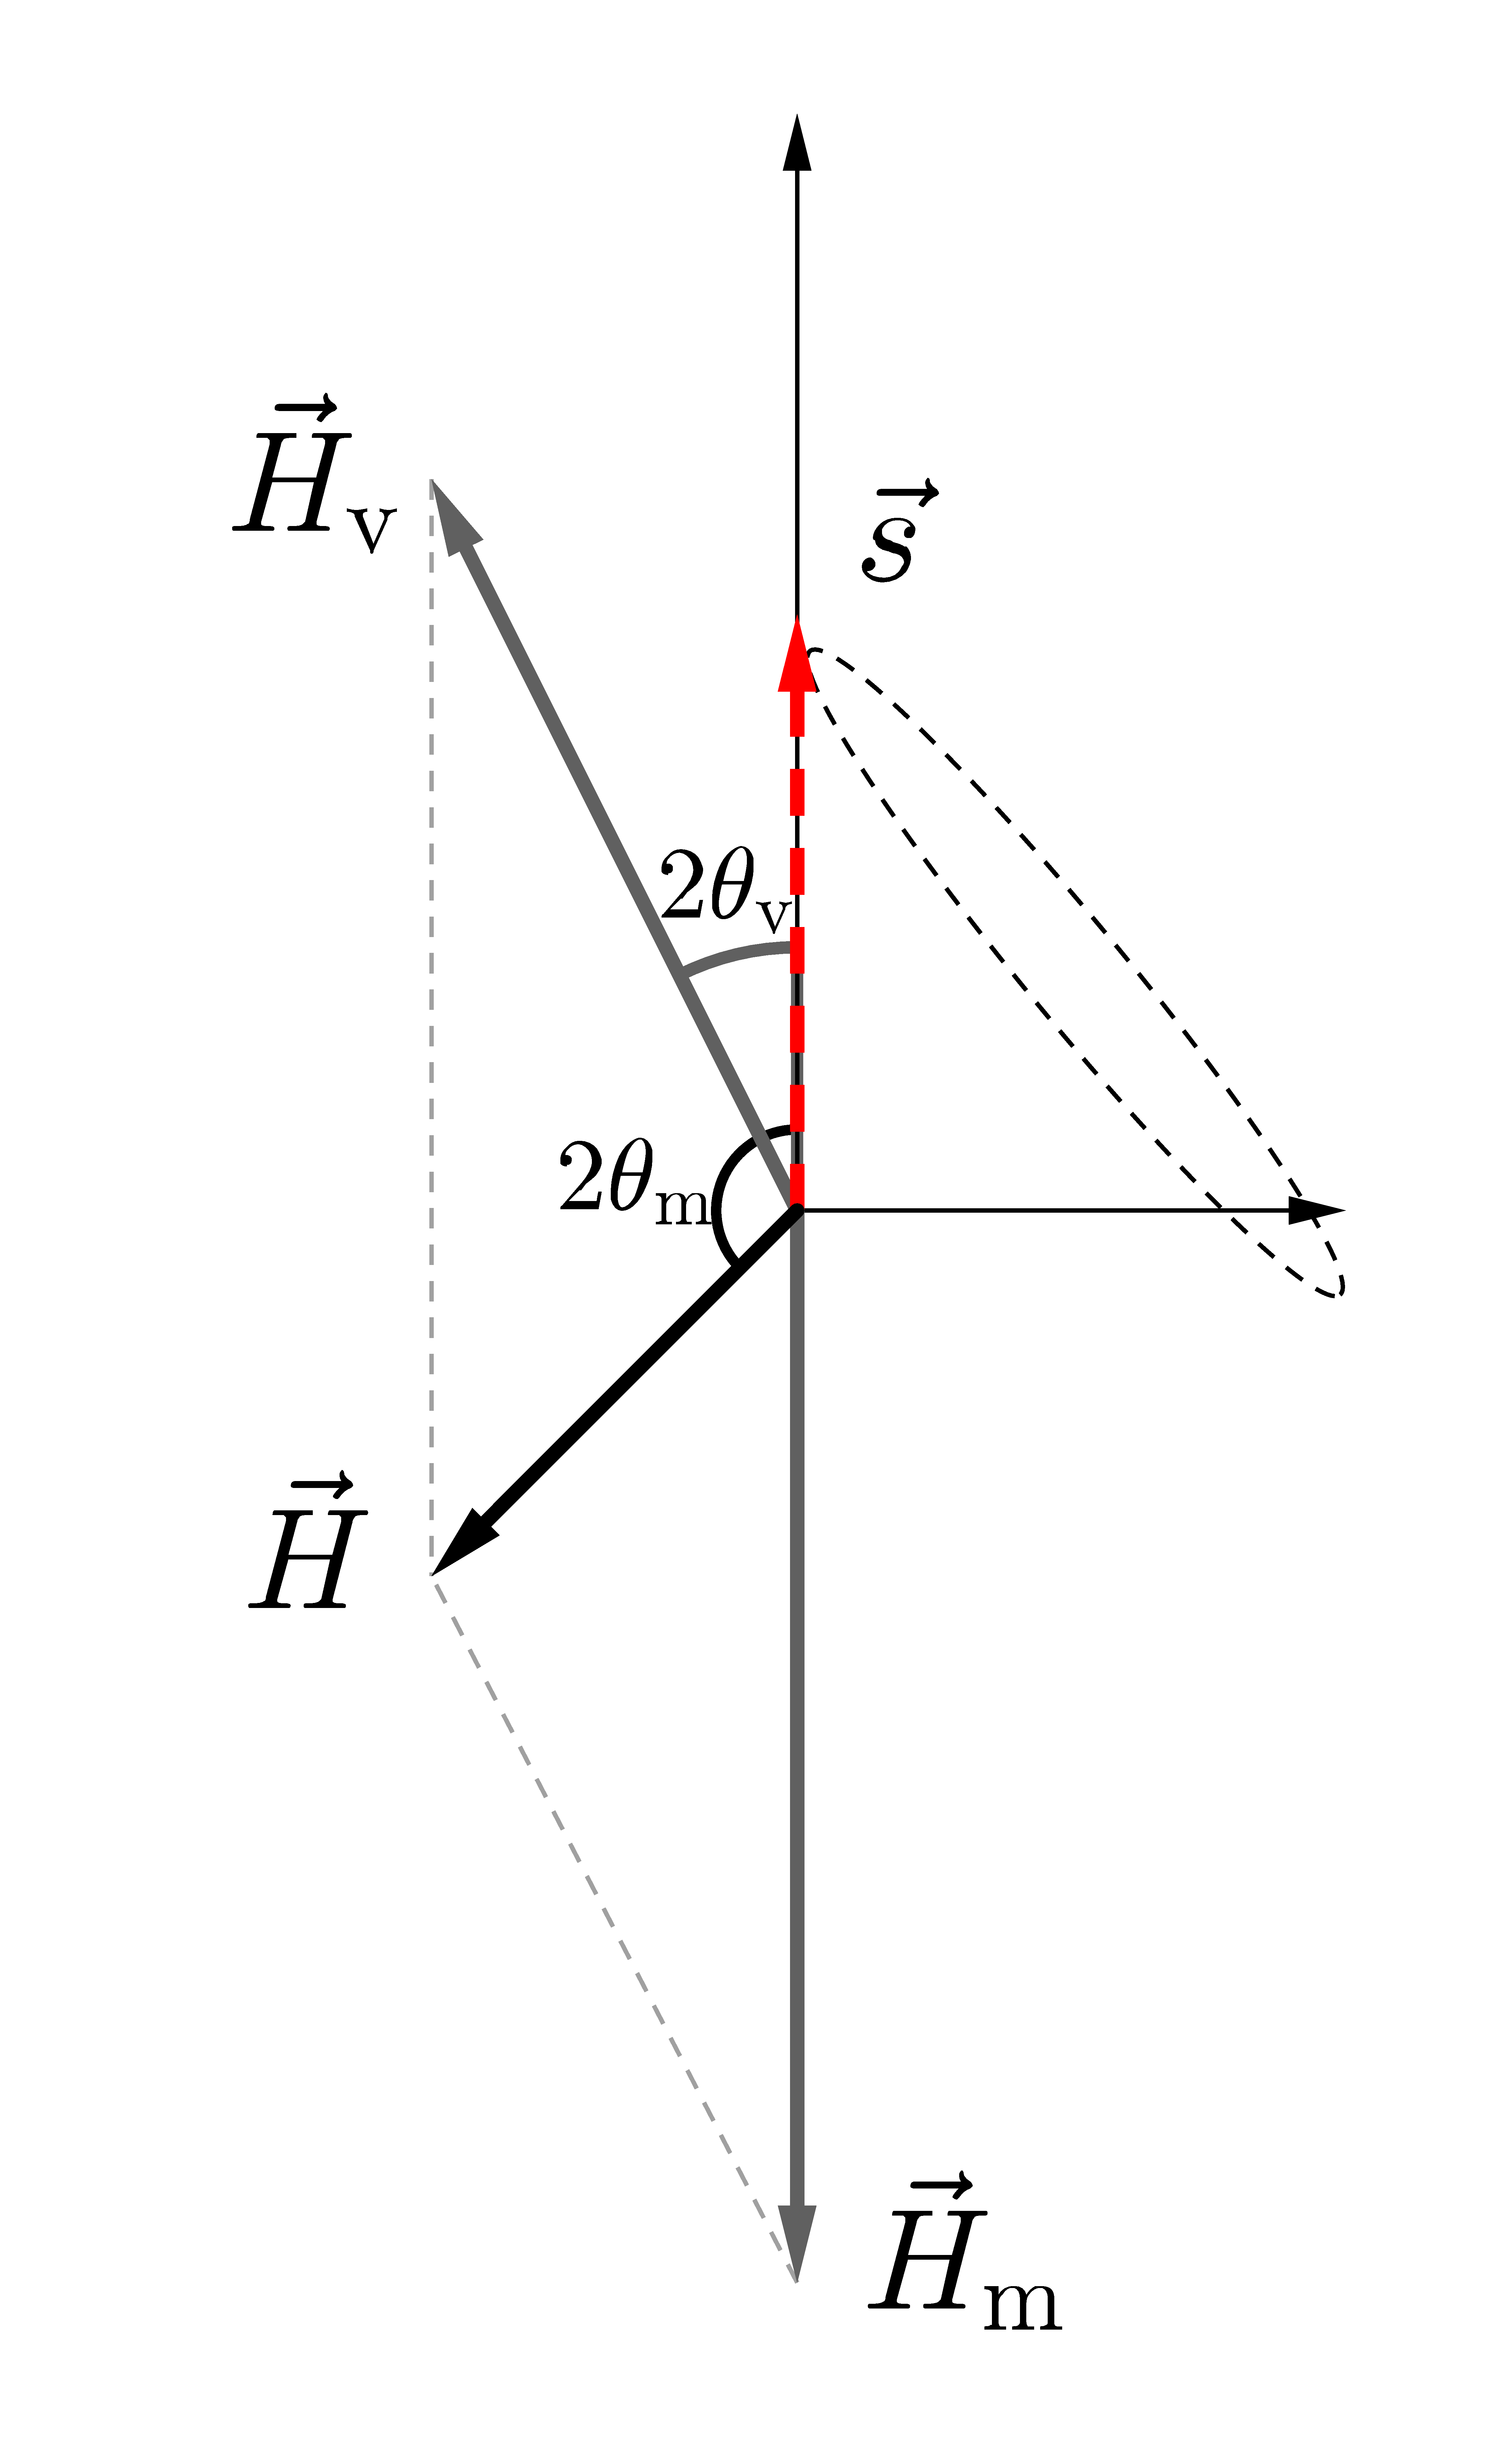
\includegraphics[width=0.4\textwidth]{chapters/assets/matter/matter-effect-notsolarge-density}
    \caption{Neutrino oscillations in flavor isospin picture with the presence of matter potential. The flavor isospin is denoted as red-dashed arrow. The two gray vectors stand for the vacuum Hamiltonians $\vec H_{\mathrm v}$ and matter potential $\vec H_{\mathrm m}$.}
    \label{chap:basics-sec:flavor-isospin-pic-fig:matter-effect-notsolarge-density}
\end{figure}

The MSW effect can also be easily explained using the flavor isospin picture. The Hamiltonian for the neutrino flavor evolution in the presence of dense matter is
\begin{align}
    &\mathsf H^{(\ff)} =  \frac{\omega_{\mathrm{v}}}{2}\left( - \cos 2\theta_{\mathrm{v}} {\sigma_3} + \sin 2\theta_{\mathrm{v}} {\sigma_1} \right)   + \frac{\lambda(x)}{2} {\sigma_3} \\
    \Rightarrow &\vec H =  \vec H_{\mathrm v} + \vec H_{\mathrm m}(x)
     = \omega_{\mathrm v}\begin{pmatrix}
    - \sin 2\theta_{\mathrm v} \\
    0 \\
    \cos 2\theta_{\mathrm v}
    \end{pmatrix}   + \begin{pmatrix}
    0\\
    0\\
    - \lambda(x)
    \end{pmatrix}  ,
\end{align}
where $\vec H_{\mathrm v}$ is the vacuum Hamiltonian, and $\vec H_{\mathrm m}(x)$ is the matter potential. The precession motion of the flavor isospin of the neutrino in the presence of dense matter is visualized in Fig.~\ref{chap:basics-sec:flavor-isospin-pic-fig:matter-effect-notsolarge-density}. The MSW resonance condition in Eqn.~\eqref{chap:basics-eqn:msw-resonance} corresponds to the scenario that the overall ``Hamiltonian vector" $\vec H$ is perpendicular to the third axis in flavor space. In this case, the flavor isospin rotates in the plane spanned by the second and third axes which gives maximum flavor oscillations (see~Fig.~\ref{chap:basics-sec:flavor-isospin-pic-fig:msw-adiabatic-critical}).

\begin{figure}[h!t]
    \centering
    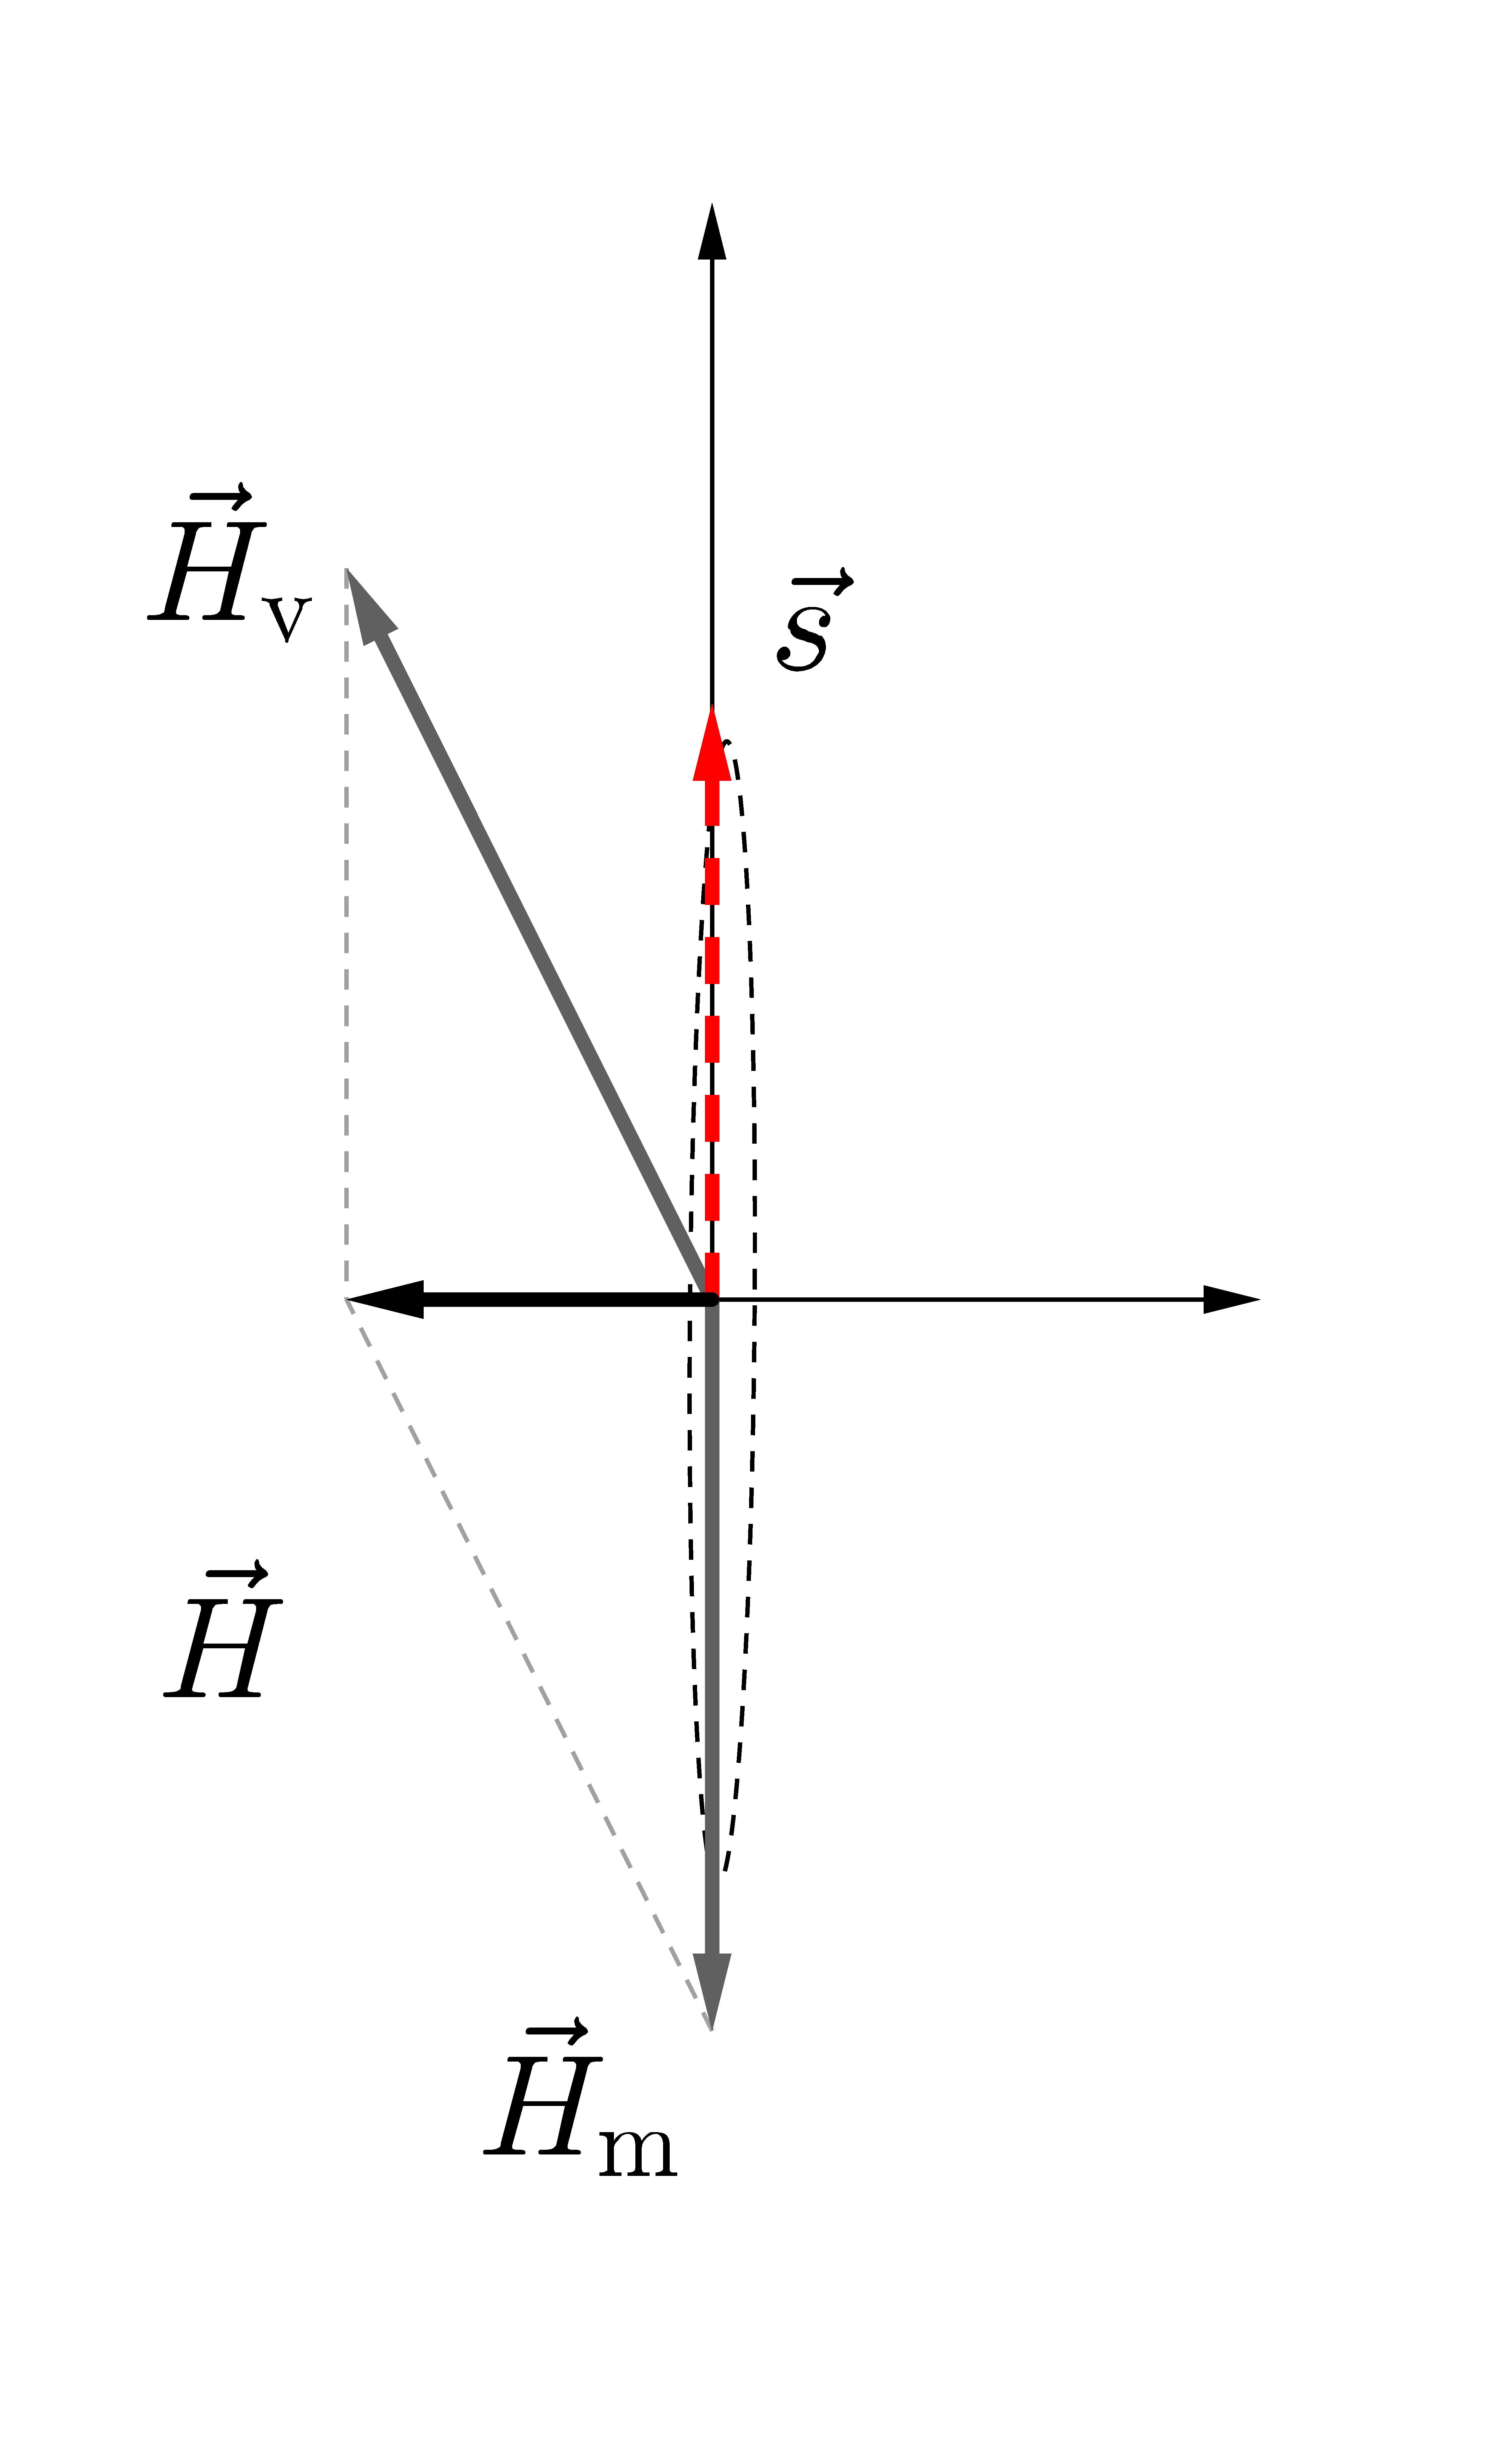
\includegraphics[width=0.4\textwidth]{chapters/assets/basics/matter-effect-critical-density}
    \caption{MSW resonance occurs when Eqn.~\eqref{chap:basics-eqn:msw-resonance} is satisfied.}
    \label{chap:basics-sec:flavor-isospin-pic-fig:msw-adiabatic-critical}
\end{figure}


The adiabatic flavor evolution of the neutrino in a varying matter density profile discussed in Sec.~\ref{chap:matter-sec:solar-neutrinos} can also be easily understood in the flavor-isospin picture.
In the region where the matter density is high, the total ``Hamiltonian vector" $\vec H$ points ``downward'' in flavor space. Therefore, a neutrino produced in the electron flavor will experience very little oscillations because its flavor isospin $\vec s$ is almost anti-parallel to $\vec H$ (see Fig.~\ref{chap:basics-sec:flavor-isospin-pic-fig:msw-adiabatic-large-density}). If the matter density along the propagation trajectory of the neutrino decreases slowly, $\vec s$ will stay almost anti-parallel to $\vec H$ as $\vec H$ rotates (see Fig.~\ref{chap:basics-sec:flavor-isospin-pic-fig:msw-adiabatic-medium-density}).
When the neutrino reaches the region with very low matter density, its flavor isospin becomes almost anti-parallel to $\vec H_{\vv}$, which implies that the neutrino is in $\ket{\nu_2}$ (see Fig.~\ref{chap:basics-sec:flavor-isospin-pic-fig:msw-adiabatic}).




\begin{figure}[htbp]
	\centering
	\begin{subfigure}[t]{0.3\textwidth}
		\centering
		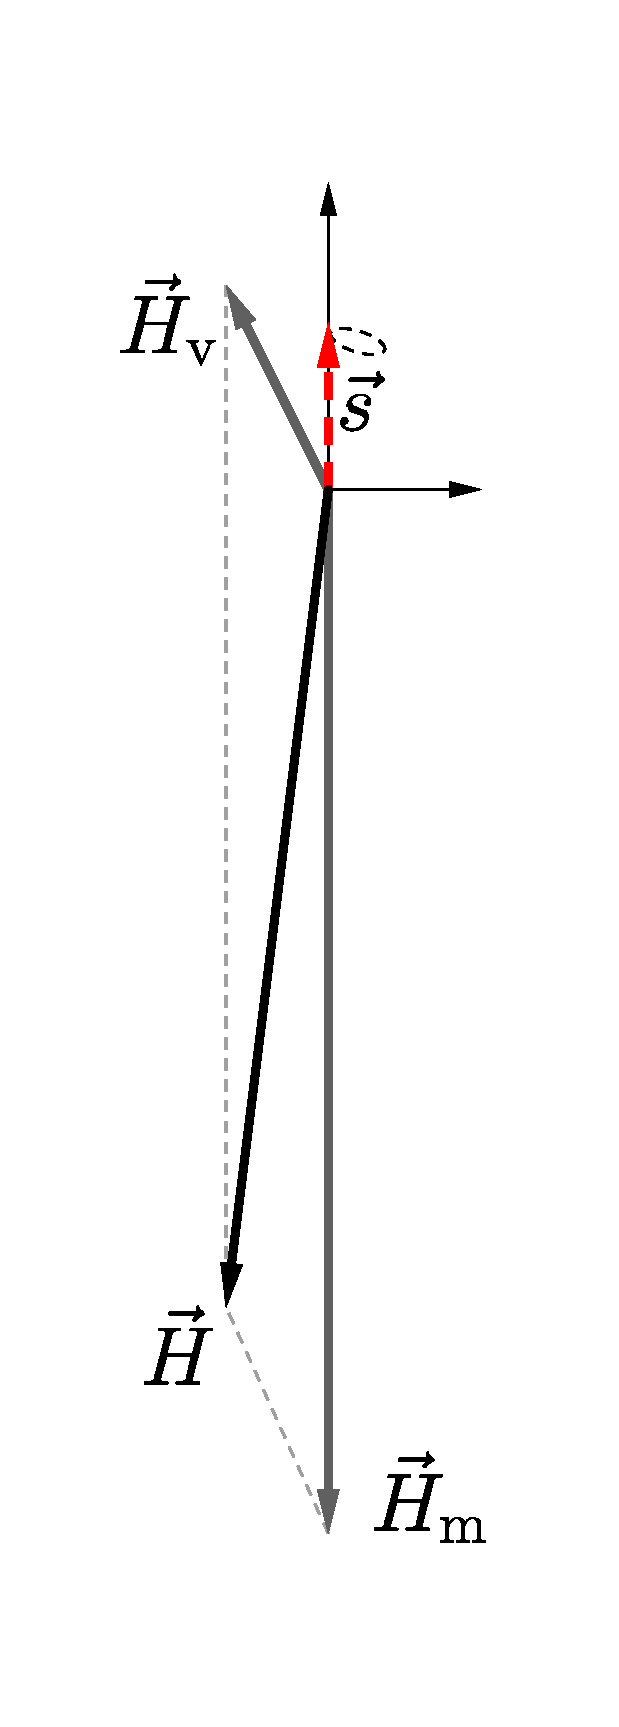
\includegraphics[width=0.8\textwidth]{chapters/assets/matter/matter-effect-large-density}
		\caption{High matter density}\label{chap:basics-sec:flavor-isospin-pic-fig:msw-adiabatic-large-density}
	\end{subfigure}%
	\begin{subfigure}[t]{0.3\textwidth}
		\centering
		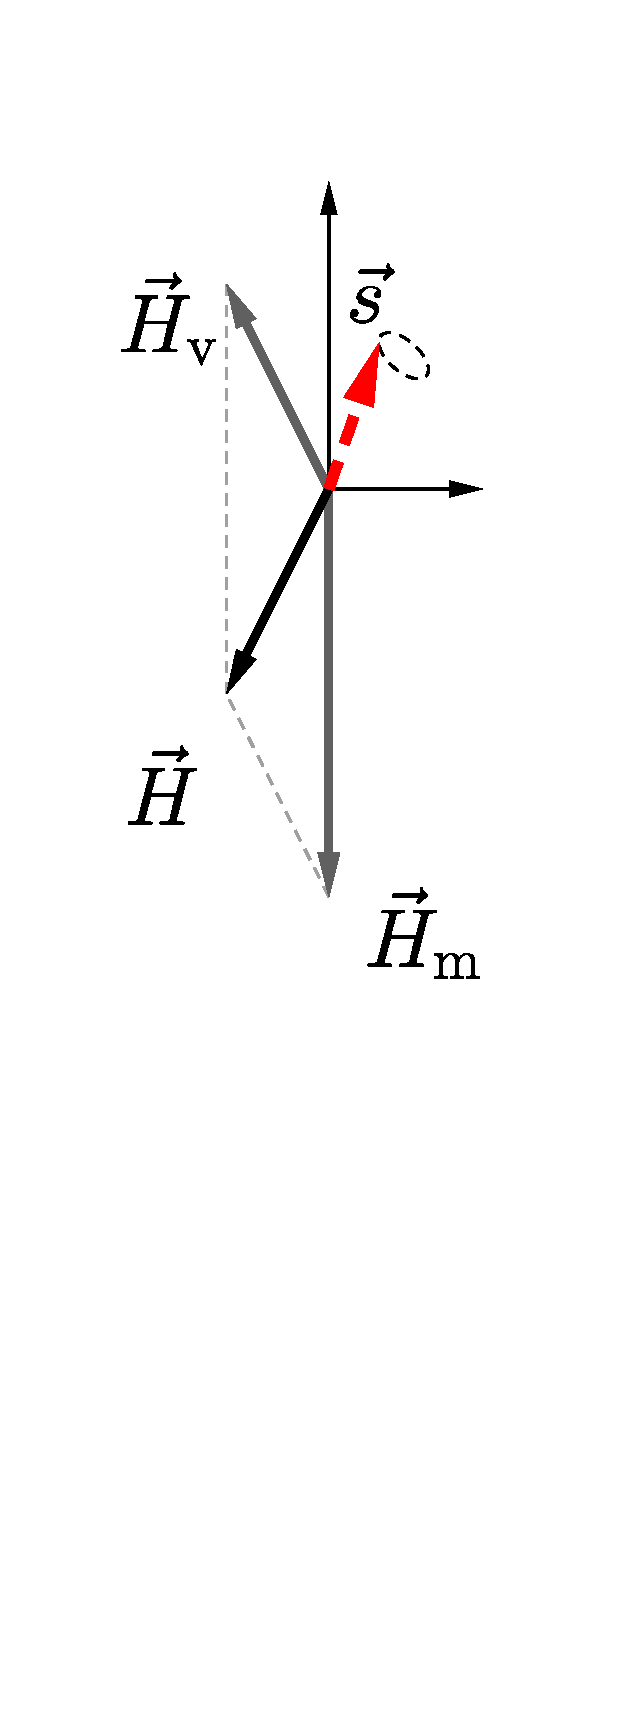
\includegraphics[width=0.8\textwidth]{chapters/assets/matter/matter-effect-adiabatic}
		\caption{Medium matter density}\label{chap:basics-sec:flavor-isospin-pic-fig:msw-adiabatic-medium-density}
	\end{subfigure}%
	\begin{subfigure}[t]{0.3\textwidth}
		\centering
    \vspace*{-3.93in}
		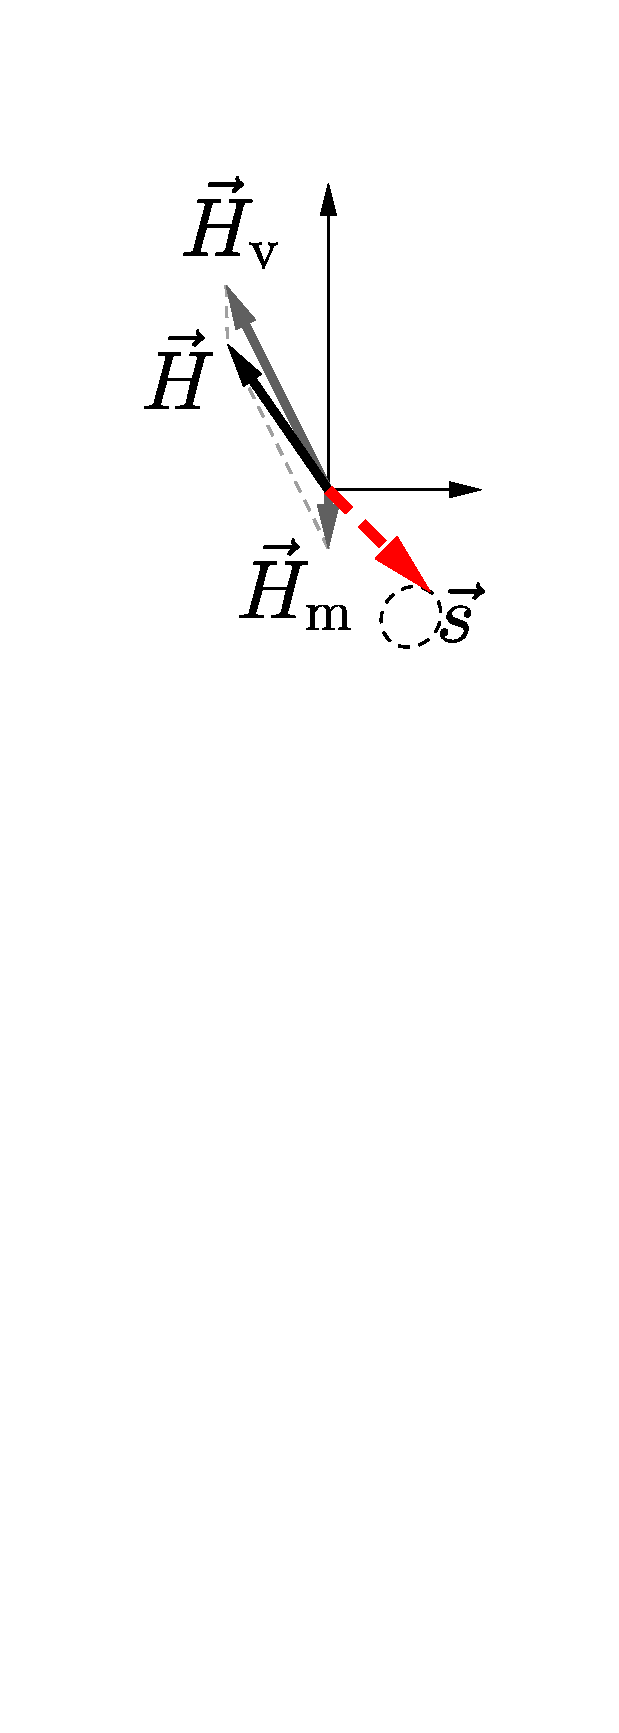
\includegraphics[width=0.8\textwidth]{chapters/assets/matter/matter-effect-adiabatic-3}
    \vspace*{-0.05in}
		\caption{Low matter density}\label{chap:basics-sec:flavor-isospin-pic-fig:msw-adiabatic-small-density}
	\end{subfigure}
	\caption{Flavor isospin picture of neutrino oscillations in matter. $\vec H_{\mathrm v}$ is the vacuum Hamiltonian, and $\vec H_{\mathrm m}$ is the matter potential.}\label{chap:basics-sec:flavor-isospin-pic-fig:msw-adiabatic}
\end{figure}






\section{Summary}

Neutrino oscillations in vacuum and in matter with a smooth profile have been explained. The neutrino oscillation phenomenon reveals a secret of the nature of the neutrino, i.e., its flavor states are not the same as the mass eigenstates of the Hamiltonian.
As a result, a neutrino produced in the pure flavor state through weak interaction will not remain in the same flavor state as it propagates, but oscillates between different flavors. The problem of neutrino oscillations in an environment with rapidly varying matter densities is significantly more difficult than that in a smooth profile. This will be discussed in the next chapter.

%!TEX root = ../dissertation.tex
\chapter{Conclusion}
\label{conclusion}

We conclude that neutrinos oscillate.


% the back matter
% \backmatter

\printbibliography

%\clearpage
%\bibliography{references}
%\addcontentsline{toc}{chapter}{References}
%\bibliographystyle{apalike2}


%\bibliographystyle{AMS}
%\bibliography{bibfile_name}

\end{document}
